\documentclass[math]{cours}
\author{Jean-Louis Halpérin}
\title{Introduction au Droit Public Français}
\date{2024-2025}
\begin{document}
\bettertitle

\section*{Informations}
Site du cours: \url{www.droit.ens.fr}\\
Chaque semaine, préparer un exposé sur l'arrêt (3mn au début) pour progresser. 2h de cours + 1h de review de décisions de justice.\\
Adresse: \url{mailto:jean-louis.halperin@ens.fr}

\section{L'Ordre Judiciaire}
\subsection{Les règles de droit}
	Définition essentialistes du droit et définition formalistes: Le droit est avant tout une technologie, définition dite positiviste.
	On définit une règle de droit comme ce qui est reconnu par une juridiction, par un jury.
	Hermann Kantovitch appelle ceci le critère de justiciabilité: la règle de droit, c'est ce qui est reconnu par des juges.
	On répond à cela que s'intéresser aux décisions judiciaires c'est s'intéresser à la pathologie du droit.
	Heureusement, il n'y a pas que des situations qui sont contestées.
	Il y a toutes formes de situations juridiques qui se déroulent sans procès.
	De même que les médecins apprennent l'anatomie au travers des maladies, on apprend le droit à travers ses problèmes. \\

	En France il y a deux ordres juridictionnels:
	\begin{enumerate}
		\item L'ordre judiciaire (civil et pénal), juridiction judiciaire, juge judiciaire. Au sommet: la cour de cassation.
		\item L'ordre administratif, avec les juridictions administratives. Au sommet: le conseil d'état.
	\end{enumerate}
	Au dessus de ceci se situe le \emph{Tribunal des Conflits}, qui arbitre lorsqu'il y a un conflit et qu'on ne sait pas quelle juridiction doit la décider.
	Il ne s'agit pas d'une cour suprême qui décide notre droit.
	Le Conseil Constitutionnel n'est pas une cour constitutionnelle, il ne rend que des décisions, et si elles ont beaucoup d'influence, il ne peut pas casser un arrêt de la cour de cassation ou du conseil d'état.
	Ce n'est par exemple pas le cas en Allemagne.
	Le Conseil Consitutionnel est en dehors de l'organisation juridictionnelle, même s'il entretient des rapports forts avec celle-ci.

	Il y a une hiérarchie au sein des ordres juridictionnels, les \emph{cours} se situent au dessus des \emph{tribunaux}.
	Les tribunaux rendent des \emph{jugements} et les cours rendent des \emph{arrêts}.
	On peut parler de \emph{décision} judiciaire pour tout tribunal sans être propre, mais c'est le terme technique (et le seul donc) qui peut être employé pour le Conseil Constitutionnel.
	Attention: en droit, tout est arbitraire et décidé par un législateur. \\

	Les cours peuvent être classées en différentes juridictions (civile et pénale ou répressive).
	La distinction se fait notamment sur les parties au procès:
	\begin{description}
		\item[Au Civil] Il y a au moins deux personnes (privées).
		\item[Au Pénal] Il oppose toujours l'état (représenté par le ministère public) à une personne qui est \emph{oursuivie}.
	\end{description}
	Le procès administratif a en général lieu entre une personne et un acte, et non contre un fonctionnaire ou l'état comme personne morale.
	Les juridictions pénales jugent les causes qui relèvent du droit pénal, qui sont en grande partie (mais pas en totalité) énuméré dans le code pénal (code Badinter qui a remplacé le code Napoléonien).
	Il y a des lois en dehors du code, par exemple la loi sur la presse.
	Les règles pénales répriment ce qu'on appelle des infractions.
	Les infractions sont divisées en trois niveaux:
	\begin{enumerate}
		\item Les contraventions (de police) qui ne peuvent être punies que d'une peine d'amende
		\item Les délits qui peuvent être punis d'amendes plus lourdes et d'emprisonnement jusqu'à 10 ans
		\item Les crimes qui sont punissables, outre des amendes, de réclusion criminelle entre 15, 20, 30 ans et perpétuité.
	\end{enumerate}
	Les peines présentées dans le code pénal sont les peines maximales, que le juge ne peut pas dépasser.
	Il n'y a pas lieu de s'étonner sur le fait que les peines ne soient pas toujours maximales, en vertu de l'individualisation du droit.
	Le terme délit est un des termes les plus équivoques qui soient:
	\begin{enumerate}
		\item Infractions jugées par le tribunal correctionel, niveau entre les contraventions et les crimes
		\item En droit pénal, peut désigner l'ensemble des infractions
		\item En matière de responsabilité civile (pour obtenir des dommages et intérêts), on parle de \emph{délit civil}.
	\end{enumerate}
	Le terme d'\emph{infraction} qui vient du verbe latin \emph{infringere} (on dit que les contrevenants à la loi, violent la loi).
	Cette expression est impropre.
	Par exemple, s'agissant du vol, le voleur ne viole pas les règles du code pénal, puisque celui-ci n'interdit pas de voler, mais à partir du moment où il est poursuivi, déclenche l'application des règles du code pénal.
	Les voleurs ne violent pas la loi, mais en déclenchent l'application.
	Dans la définition du procès pénal, les magistrats du ministère public (partie des magistrats: procureur, vice-procureur, substitut du procureur), souvent qualifié de magistrats du \emph{parquet}, ont le quasi-monopole de la poursuite.
	Quasi-monopole car certaines administrations (ponts et chaussées, eaux et forêts, bois\ldots) ont dans leurs attributions la capacité de donner des contraventions.
	Le parquet agit principalement sur des informations fournies par des personnes qui dénoncent des infractions ou s'en plaignent.
	La \emph{dénonciation} est l'acte d'informer le procureur de la République de la connaissance d'une infraction que l'on juge devoir être punie.
	La dénonciation n'est pas une \emph{délation}, et est même quelque chose d'honorable.
	Elle peut être faite par la victime elle-même (qui a plutôt intérêt à porter plainte) ou par n'importe quel tiers.
	Il n'y a pas d'obligation de dénonciation, sauf pour les autorités constituées, c'est à dire les fonctionnaires publics cf Article 40 du code de procédure pénale.
	Les fonctionnaires ont l'obligation de dénoncer ce qu'ils voient dans \textbf{l'exercice de leurs fonctions}.
	Une interprétation toutefois peut dire qu'une accusation ne peut pas se faire par ouï-dire.
	Certaines autres interprétations disent qu'il faut repasser par le chef d'établissement et d'autres qu'il ne faut agir qu'en considération de la victime.
	C'est une obligation qui n'est pas sanctionnée pénalement, et qui est rarement (presque jamais) sanctionnée disciplinairement.
	Ce n'est pas le seul cas d'une obligation non sanctionnée.\\

	L'audition d'une dénonciation se fait en commissariat ou en gendarmerie et peut donner lieu à une main courante ou à une plainte (appelée plainte simple).
	Le ministère public a le pouvoir de trancher sur l'opportunité des poursuite:
	pour toutes les dénonciations et plaintes, le ministère public a la possibilité de les classer sans suite,
	ou parce que le fait délictueux (au sens général) est mal établi, que le fait ne constitue pas une infraction,
	que le ministère public juge qu'il n'est pas bonne politique de poursuivre ce genre de fait.
	Il est possible de vaincre le classement sans suite en portant plainte avec constitution de partie civile:
	la constitution de partie civile peut avoir lieu à n'importe quel moment dans la procédure pour réclamer des dommages et intérêts.
	La victime a le choix soit d'aller au civil en parallèle de la procédure pénale soit de se constituer partie civile.
	En début de procédure, la plainte avec constitution de partie civile oblige un juge d'instruction à lancer une instruction et force le ministère public à agir.
	Toute constitution de partie civile est accompagnée d'une consignation d'une somme d'argent qui vise à informer la personne qui se constitue partie civile de la gravité de la procédure, et en cas de relaxe ou d'acquittement, à qualifier la dénonciation de calomnieuse.
	Sur ces bases, le ministère public lance l'enquête via la police judiciaire.
	Il y a deux types d'enquêtes en France:
	\begin{enumerate}
		\item Enquête de \emph{flagrant délit}: quand le délit vient de se commettre et qu'il y a des témoins/des preuves.
			La police peut alors perquisitionner sans l'accord de la personne perquisitionnée entre 6h et 21h.
		\item Enquête \emph{préliminaire}: quand la police est informée par des dénonciations, plaintes ou son travail de surveillance et qu'elle repère quelque chose.
			Les pouvoirs des policiers sont plus faibles.
			Les perquisitions doivent notamment être autorisées par la personne.
	\end{enumerate}
	Depuis l'extrême fin du 20$^{e}$ siècle, il y a nombre de procédures alternatives pour éviter les tribunaux:
	\begin{itemize}
		\item Classement sans suite
		\item Prononciation d'une amende forfaitaire: pas de procès, constatation dans le procès-verbal par l'officier de police judiciaire.
			Si la personne accepte de payer, le montant est fixé entre 11 et 3000€.
			Sinon, ce qui arrive en moyenne 10 millions de fois par an, on entre dans le cas de l'amende forfaitaire majorée.
		\item L'ordonnance pénale (depuis 1999, utilisée surtout pour les délits routiers et les stupéfiants):
			le ministère public établit la sanction pour les contraventions ou pour des délits mineurs,
			la personne est informée mais ne sera pas convoquée, le juge du tribunal de police (ou correctionnel) appose simplement sa signature
		\item La composition pénale :
			sur proposition du ministère public, non nécessairement l'amende maximale mais non nécessairement.
			La personne est convoquée et si elle ne s'y rend pas, le juge du tribunal de police (ou correctionnel) approuve la peine proposée par le ministère public.
		\item La Comparution Avec Reconnaissance Préalable de Culpabilité:
			la personne est convoquée et peut faire valoir son argument (souvent avec son avocat),
			le ministère public propose une peine inférieure à celle maximale en échange de la reconnaissance de culpabilité.
			Le président du tribunal correctionnel habilite la procédure.

		\item Le cas le plus classique:
			à l'issue d'une enquête de PJ, on prévient la personne visée (le prévenu) et il y a un procès.
		\item La comparution immédiate (flagrant délit):
			Enquête très rapide et comparution dans les quelques jours.
			La personne peut refusée d'être jugée si rapidement.
			Il n'y a pas de décision de comparution immédiate sans l'accord (un peu contraint) de la personne prévenue.
	\end{itemize}
	Les statistiques judiciaires sont sous forme d'une brochure qui donne les chiffres de 2 ans auparavant appelées \textit{Les chiffres-clefs de la justice}.
	Il y a aussi un petit peu de propagange appelée \textit{La Réponse Pénale}.
	Le non-lieu, l'absence de jugement et le classement sans suite sont considérées comme des réponses pénales.
	En 2022: il y a 648889 décisions pénales, 83\% des tribunaux correctionnels, 5\% des tribunaux de police pour 1800000 décisions civiles.\\

	Il y a 8800 magistrats en France. La loi Dupont-Moretti prévoit une augmentation du nombre de postes.
	Les magistrats sont des fonctionnaires dont le statut particulier est régi par une ordonnance de 1958.
	Il y a un seul statut, un seul corps, mais des positions diverses dans la carrière:
	ou bien dans le siège ou bien dans le parquet.
	La plupart des magistrats alternent dans leur carrière, mais ne peuvent occuper les deux à la fois.
	Les magistrats dépendent du Conseil Supérieur de la Magistrature, dernièrement révisé en 2008 (application en 2011).
	Le CSM n'est plus présidé par le Président de la République.
	Il est composé de deux formations, une pour ceux du siège et une pour ceux du ministère public.\\

	La formation compétente pour les magistrats du siège comporte 7 magistrats, le Premier, 6 magistrats élus, un conseiller d'état élu par ses pairs, un avocat élu par le Conseil national du barreau, et 6 personnalités qualifiées nommées.
	Concernant la formation des magistrats, le CSM fait une proposition au Président de la République.
	Le CSM choisi les magistrats supérieurs (par ancienneté dans la carrière souvent).
	Pour les autres magistrats, le ministère de la justice fait une proposition, et le CSM doit l'accepter par ce qu'on appelle un \emph{avis conforme}.
	Un avis peut être \emph{simple} que l'autorité qui demande l'avis n'est pas tenue de suivre, ou \emph{conforme} auquel cas l'autorité concernée par l'avis est tenue de suivre.
	C'est aussi cette formation qui est compétente pour juger les magistrats du siège selon les manquements dans leurs fonctions.
	Le ministère est tenu de suivre cet avis.\\
	La formation du parquet comporte 5 magistrats du parquet, un du siège et les 8 mêmes non-magistrats que celle du siège.
	En matière de nomination, le CSM fait des propositions que le président de la république n'est pas juridiquement tenu de suivre.
	En matière disciplinaire, la formation des magistrats du parquet rend un avis que le ministère n'est pas tenu de suivre.

\subsection{Formation des Tribunaux}
	Les Lois Taubira, Belloubet et LOPJ (loi Dupont-Moretti) ont réformé le système de tribunaux français.
	La loi Belloubet de 2019 a fusionné les Tribunaux de Grande Instance (TGI) et Tribunaux d'Instance.
	On parle maintenant de Tribunaux Judiciaires (TJ). Il y en a 164 dans les villes où siégaient un TGI et TI.
	Il y en a au moins un par département.
	Le TJ est, en matière civile, la juridiction de droit commun (qui règle le plus grand nombre d'affaires).
	D'abord pour les affaires personnelles et mobilières au dessus de 10000€, l'état des personnes (mariage, PACS, naissance, nationalité), la propriété immobilière, les brevets, les grèves\ldots
	Les TJ ont rendu 1,4 millions de décisions en 2022.
	Ils siègent en général à 1 ou 3 juges, mais il y a de plus en plus de procédures à 1 juge ou sans audience.
	Le président est juge des référés (référé civil, procédure d'urgence qui ne va pas rentrer dans les détails de l'affaire, qui va accorder une provision, interdire une publication.). Il y a eu 105000 décisions en référé en 2022.
\begin{figure}[h]
	\centering
	\begin{tikzpicture}
		\node{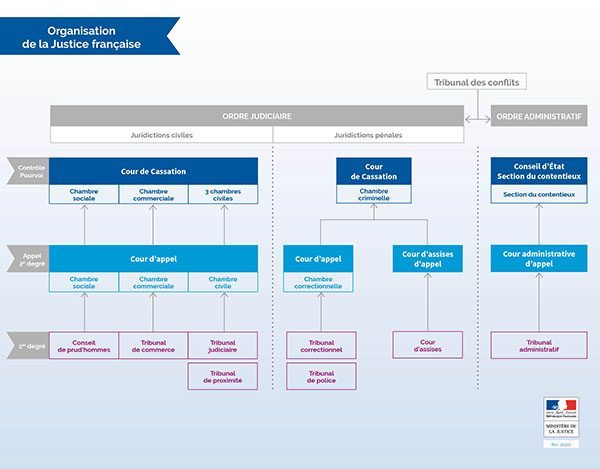
\includegraphics{orga_juridictionnelle}};
	\end{tikzpicture}
	\caption{L'organisation juridictionnelle -- Source: Ministère de la Justice}
	\label{fig:orga_juridictionnelle}
\end{figure}
	Dans 125 villes françaises qui avaient un TI mais pas de TGI, ont été maintenus des Tribunaux de Proximité (TP).
	Des juges du contentieux de la protection (JCP) y décident des affaires de surendettement, de crédit à la consommation, de bail d'habitation, de protection des majeurs, d'explulsion.
	Les JCP jugent à juge unique.\\
	Les contraventions des 5 classes sont jugées par les tribunaux de police (53000 jugements pour les 4 premières classes), auxquelles s'ajoutent les décisions d'ordonnance pénale.
	Les tribunaux correctionnels jugent les délits (avec des peines d'amende >3500€ et/ou de l'emprisonnement jusqu'à 10 ans).
	Depuis 2020, les peines de prison de moins d'un mois ne peuvent plus être prononcées\footnote{Il y a 85000 personnes dans les prisons françaises, pour 59000 places. La justice pénale française n'est donc pas laxiste.}.
	Les TCs peuvent produire des sanctions alternatives (bracelet électronique, travaux d'intérêt généraux\ldots). Ils rendent 580000 décisions par an.\\
	Toujours rattachés aux TJ, les juges d'instruction instruisent les crimes et les délits complexes (cumul d'infraction, délit nécessitant une instruction permettant de poursuivre l'enquête par une mise en examen).
	Depuis 2000 et la loi sur la présomption d'innocence, le juge d'instruction ne peut plus procéder à une décision de détention provisoire, et doit alors décider avec le juge des libertés et de la détention provisoire.
	C'est en principe une exception en cas de risque pour l'ordre public, les biens ou les personnes.\\
	Les juges des enfants siègent seuls ou dans l'un des 155 tribunaux pour enfants (avec 2 assesseurs non-professionnels).
	Le régime de traitement des mineurs est spécifique et existe depuis 1810 dans le code pénal ainsi que dans d'autres textes.
	Il existe également deopuis 2021 un code de la justice pénale des mineurs.
	Il a clarifié la question de la responsabilité ou de l'irresponsabilité pénale des mineurs.
	Il y a une distinction fondamentale qui est faite entre les mineurs discernents ou non-discernents.
	Être discernent c'est avoir conscience du fait de commettre un acte grave et d'avoir conscience de la sanction.
	Le code de 2021 établit la présomption qu'il n'y a pas de discernement du mineur avant 13 ans.
	À ce titre, les mineurs de moins de 13 ans sont présumés non-discernents et donc exempts de responsabilités.
	Au contraire, les mineurs de 13 à 18 ans sont présumés discernents.
	En chambre du conseil (à huis clos), pour les contraventions de 5ème classe et certains délits, le juge des enfants peut prononcer à l'égard des mineurs à partir de 10 ans et jusqu'à 13 ans des sanctions dites éducatives.
	Le mineur, s'il n'est pas en danger reste de sa famille, mais peut aussi être retiré à sa famille et placé en famille d'accueil, sous la tutelle de l'état ou dans un centre spécialisé.
	À partir de 13 ans, les mineurs peuvent être envoyés en prison, dans des centres éducatifs fermés, le code pénal prévoit des peines pour les mineurs réduites de moitié.
	Il y a des exceptions, notamment pour les grands mineurs (16-18 ans) récidivistes.
	Pour les crimes des mineurs entre 16 et 18 ans, la cour d'assises des mineurs. \\
	Il y a 134 tribunaux de commerce qui jugent les conflits entre commerçants (personne publiques inscrites au registre du commerce) ou des sociétés relatifs à des actes de commerce (\textit{faillite}, mot qui n'a plus de sens depuis les années 60).
	Les juges sont élus pour 4 ans par les commerçants et ont rendus 109000 décisions en 2022.\\
	Les conseils de prud'hommes (211 au lieu de 271 avant 2008) jugent les litiges individuels du travail.
	Les juges sont désignés en 5 sections (industrie, commerce, culture, professions libérales, cadres\ldots) siègent de manière paritaire en bureau de conciliation (au moins 2) ou de jugement (au moins 4).
	Ils comptent autant de représentant des employés que des patrons.
	Ils ont rendu 113000 décisions en 2022.\\
	Les 272 tribunaux paritaires des baux ruraux règlent les conflits sur les baux ruraux sont des juridictions avec des juges élus par les représentants syndicaux des propriétaires et locataires de baux et sont placés sous la présidence d'un juge professionnel.
	On appelle ce type de juridiction avec des professionnels et non-professionnels des juridictions \emph{d'échevinage}.\\
	La cour d'assises (avec la cour criminelle départementale) sont composées (en première instance) de 3 magistrats professionnels et de 6 jurés (9 en appel) tirés au sort.
	Il y en a une par département, c'est une formation temporaire (qui juge par session).
	Les cours d'assises jugent de crimes (réclusion de 15 ans à perpétuité).
	Les personnes traduites devant une cours d'assises s'appellent \emph{accusées} et non prévenues.
	Magistrats et jurés délibèrent ensemble et sur la culpabilité et sur la peine.
	Les cours départementale criminelles (ou tribunaux criminels) devant lesquelles sont jugés les crimes passibles de réclusion criminelle de 15 et 20 ans (par exemple les viols).
	Les tribunaux criminels n'ont pas de jury et sont composés de 5 magistrats, mais suivent la même procédure.
	Les peines criminelles peuvent être accompagnées d'une peine incompressible de sûreté durant laquelle aucune réduction ni libération ne peut avoir lieu.
	En dehors de cette période, les réductions sont courantes et sont appliquées par le Juge d'Application des Peines (JAP).
	La perpétuité réelle existe tout de même, même si on la voit peu.\\
	Les cours d'appel sont séparées en de multiples chambres (civiles (appels des TJ mais peu des JCP), commerciales (appels des tribunaux commerciaux), sociales (appels des prud'hommes) et de l'instruction (appels des décisions prises par les juges d'instructions ou les juges des libertés et la détention)).
	Le délai d'appel est de 10 jours au pénal, 1 mois au civil.
	La décision peut être mise en suspens pendant la procédure d'appel.\\
	La cour de cassation (créée le 27 novembre 1990, sujet de la thèse de JLH) est composée d'une centaine de magistrats, composées de 6 chambres (3 civiles, une sociale, une pénale, une commerciale).
	Dans chaque chambre siègent un nombre de conseillers à la cour de cassation.
	Chaque chambre à un président et à la tête de la cour un premier président (appelée le Premier).
	Il y a un parquet auprès de la cour de cassation composé du procureur général de la cour de cassation, d'avocats généraux (ce ne sont pas des avocats mais les assistants aux procureurs généraux).
	Le pourvoi (ou recours) en cassation (procédure intentée par une partie qui a perdu en cour d'appel, qui n'est pas un troisième degré de justice),
	demande à la cour de cassation de ne pas se prononcer sur le fond de l'affaire mais sur le respect du droit par la cour d'appel.
	La cour de cassation est très sollicitée (15000 décisions au civil, 7000 au pénal).
	Par comparaison, le conseil d'état juge (9000 affaires par an).
	Depuis 2002, il y a une procédure de non-admission qui permet de rejeter les pourvois non sérieux.
	Tout pourvoi doit être soutenu par un avocat.
	Depuis 1970, pour juger des affaires plus sérieuses, on convoque l'assemblée plénière (19 membres: Premier, présidents, doyens, membres des chambres).
	Au cas où après un pourvoi en cassation et un renvoi en cour d'appel, il y a un deuxième pourvoi, ou bien il y a rejet, ou bien l'assemblée plénière juge.
	Il n'y a pas d'effet suspensif au civil mais au pénal si, ce qui a été très important avant l'abolition de la peine de mort.
	Il y a ouverture à cassation en cas de:
	\begin{itemize}
		\item violation de la loi en cour d'appel,
		\item violation des formes de procédure,
		\item défaut de base légale,
		\item excès de pouvoir
	\end{itemize}
	Toutes les décisions de justice doivent être motivés. La cour de cassation a imposé jusqu'à 2019 le style classique et laconique des décisions.
	La motivation d'une décision de justice se présente sous une phrase commençant par \textit{Attendu que} et comportant de nombreuses subordonnant.
	Elle doit contenir un visa, i.e. l'évocation d'un texte de loi.
	On utilise désormais un style plus direct pour les attendus. \\
	En France, la jurisprudence désigne les décisions judiciaires qui tranchent un procès et posent une norme individuelle (qui ne concerne que les parties au procès) et qui vont d'une certaine manière servir de précédent, être imitées, reprises et être transformées en une norme globale.
	Les tribunaux créent du droit par la jurisprudence.
	Tous les énoncés de droit demandent à être interprétés et appliqués, et la norme est donc créée par l'interprétation et donc par la décision judiciaire.
	L'article 5 du code civil (inchangé depuis 1804) interdit à toute juridiction de créer des arrêts de réglement.
	Le même code civil dit dans l'article 4 que le juge qui ne tranche pas un procès commet une faute grave.
	Le juge ne peut pas s'abriter pour éviter de trancher sur le silence ou l'obscurité.
	C'est le juge qui dit si un texte est clair ou non, et notamment les juges suprêmes. Ce sont eux qui posent la norme, mais pourquoi ?
	Notamment de par une loi de 1837 qui a inauguré le mécanisme de l'assemblée plénière qui force la cour d'appel à suivre la décision de l'assemblée plénière.
	Certains disent que le législateur laisse aussi faire, parce que les parlementaires n'y connaissent rien.
	Ainsi, certaines normes individuelles sont transformées en normes générales.

\subsection{Etudes de Décisions}
\subsubsection{Etude d'une décision de la 1ere Civ du 9 Oct 2001}
	Voir \ref{CassCiv19102001}
	M. Franck X a perdu devant la cour d'appel.
	La naissance a eu lieu en 76, la décision en 2001. Il n'y avait pas prescription, celle-ci étant suspendue pendant la minorité de l'enfant.
	La cour de cassation n'a pas obligation de répondre à tous les moyens (subdivision de l'argumentation pour ne pas mêler les reproches à la cour d'appel), même si elle l'a fait ici.
	Ici, on a une affaire civile car il s'agit d'une clinique privée, sinon, il s'agirait d'une affaire renvoyée devant le tribunal administratif à l'origine.
	La cour de cassation considère ici qu'il y a eu un vice de procédure.
	La cour de cassation considère que le médecin n'a pas rempli son contrat et casse donc la décision, la renvoyant devant la cour d'appel de Grenoble.
	Dans les années 70 (après 1975), s'est développé une jurisprudence demandant aux médecins de donner aux patients le maximum d'informations, notamment sur les risques encourus.
	Le patient ou son représentant signe alors un document précisant qu'il est bien informé.
	L'information par le médecin s'étend à des cas imprévus en cas d'opération et ne s'applique pas en état d'urgence.
	Le médecin doit continuer à informer la femme pendant l'accouchement.
	Le médecin s'est défendu en disant qu'il n'avait pas manqué à une obligation qui n'existait pas encore.\\

	Ici, le premier paragraphe explique la situation causant litige.
	Les deux suivants résument la conclusion de l'appel.
	Le dernier donne la réponse de la cour de cassation (\textit{cependant}) et son arrêt.
	La cour de cassation voit, au milieu de l'accouchement, que le médecin viole le principe constitutionnel de sauvegarde de la dignité humaine.
	Ce principe n'est pas clairement écrit dans la constitution, mais est lu entre les lignes du préambule de la constitution de 1958 qui fait référence à celui de la constitution de 1946 qui parle de la victoire contre les puissances qui ont voulu asservir l'homme.
	La jurisprudence de l'époque précisait que le médecin était dans son droit, mais la cour de cassation juge que l'interprétation jurisprudentielle ne doit pas dépendre de la période ou les faits se sont produits.
	Il faut appliquer rétroactivement une règle nouvelle qui était imparfaitement connue au moment des faits.
	\textit{Nul ne doit se prévaloir d'un droit acquis à une jurisprudence figée}, il est tout à fait possible pour la cour de cassation de changer la jurisprudence,
	et le plaideur ne peut se plaindre de la différence de jugement rendu entre deux époques différentes.


\subsubsection{Chambre Criminelle 25 Février 2014}
Dans cette décision \ref{CassCrim25022014}, la cour de cassation étudie le pourvoi de Mme Y contre la cour d'appel de Paris.
La cour d'appel avait déboutée Mme Y de sa plainte en diffamation publique en exposant dans son arrêt que:
\begin{itemize}
	\item Donner une image peu reluisante (termes \textit{fêtarde}, \textit{adepte de la chouille}) n'est pas contraire à la dignité humaine et ne caractérise pas une diffamation.
	\item Qu'utiliser des termes triviaux en les incluant dans un propos ne constitue pas un comportement déshonorant et ne caractérise pas une injure.
\end{itemize}
Sur ces deux moyens, la cour de cassation va pointer des contradictions de la cour d'appel, notamment en visant la loi 29 juillet 1881\footnote{Loi sur la liberté d'expression et la liberté de la presse}:
\begin{itemize}
	\item Donner des faits précis pouvant porter atteinte à l'honneur et à la considération caractérise le délit de diffamation publique.
	\item Le contexte d'un article de presse, même si le propos lui-même peut ne pas revêtir, dans un cercle privé, le caractère d'injure, constitue une injure et caractérise une injure publique
\end{itemize}
C'est pourquoi la cour de cassation va casser le jugement de la cour d'appel pour défaut de motifs et manque de base légale (en vertu de l'article 593 du code de procédure pénale) et renvoyer le jugement devant la cour d'appel de Versailles.
\subsubsection{Première Chambre Civile 14 Novembre 2006}
L'affaire \ref{CassCiv114111006} oppose l'association Croyances et libertés à la société GIP sur une parodie de la cène à des fins publicitaires
Dans cet arrêt, la 1ère Chambre Civile étudie deux pourvois:
\begin{enumerate}
	\item Le premier pourvoyé par GIP pour vice de procdéure et manque de de citation envers le directeur de GIP
	\item Le second pourvoyé par C\&L pour avoir déclaré recevable l'intervention de la LDH qui:
		\begin{enumerate}
			\item Par la loi du 29/07/1881, n'aurait pas dû pouvoir exercer des droits autres que ceux de la partie civile et n'aurait pas dû pouvoir défendre en justice un motif qui n'est pas celui qu'elle est habilitée à défendre (ici le respect de la DDHC).
			\item Que la cour d'appel autorisant cela a violé le code de procédure civile.
		\end{enumerate}
\end{enumerate}
À ceci, la cour de cassation répond que:
\begin{enumerate}
	\item L'avocat de la GIP ayant démontré dans ses réponses une parfaite connaissance du dossier n'a pas manqué de temps
	\item La cour d'appel:
		\begin{enumerate}
			\item a eu raison d'autorisé l'intervention de la LDH qui se basait sur la convention de sauvegarde des droits de l'homme et des libertés fondamentales
			\item a eu tort de retenir l'existence d'un trouble quand la seule parodie de la Cène est faite sur la forme de sa représentation et n'a pas pour but d'outrager.
		\end{enumerate}
\end{enumerate}
La cour de cassation rejette donc les deux pourvois, mais casse et annule la décision de la cour d'appel, à l'exception de la recevabilité de la LDH et confirme l'absence d'exception de nullité.
Toutefois, la Cour de cassation met fin au litige plutôt que de renvoyé et condamne C\&L aux dépens.

\medskip

La différence entre diffamation et injure se fait au niveau des faits.
La diffamation se base sur des faits tandis qu'une injure est liée à un propos sans base factuelle.
La loi du 29 Juillet 1881 s'applique aussi aux journaux.
L'injure et la diffamation publique sont des délits de presse (depuis quelques années uniquement des amendes jusqu'à 12000€, 45000€ dans le cas de diffamation/injure aggravée).
Diffamation et injure privées sont des contraventions sanctionnées d'une amende de première classe, soit 11€, justiciables du tribunal de police.
La différence se fait à la publication, ou s'il s'agit d'une réunion ouverte au public.
Sur internet, une injure et une diffamation contenue dans un message électronique qui s'adresse à des personnes nommément désignées est privée, ou avec une mention claire de l'appartenance à un groupe.
Dans le cadre d'une page ouverte au public, c'est un délit de presse.
Pouvant agir, le diffamé/l'injurié, mais le ministère public ne peut agir s'il ne s'agit pas d'une autorité public.
Le ministère public n'agit pas d'office.
En fonction des personnes, notamment dans le domaine politique.
Dans l'exercice de leurs fonctions, les parlementaires ne peuvent être poursuivis pour injure ou diffamation.
Le même terme injurieux, sur des critères jurisprudentiels, peut changer de qualification.
Par exemple, traiter quelqu'un de \textit{fasciste} fait partie du débat politique lorsqu'on l'adresse à une personne politique, en revanche, c'est injurieux envers un particulier.
L'auteur peut se défendre en essayant de requalifier l'injure et la diffamation, ou requalifier l'atteinte à l'honneur et à la considération.
Deuxième possibilité: l'\textit{exceptio veritatis}, lorsqu'un propos ou des faits déshonorant est prouvablement vrai.
Jusqu'en 2013, il y avait 3 limites principales: Premièrement, on n'avait pas le droit de prouver la vérité de faits diffamatoires datant de plus de 10 ans, ce qui était utile pour les faits de collaboration.
On a toute liberté d'injurier les morts, tant que cela n'a pas pour but de diffamer ou d'injurier les descendants, ce qui peut donner lieu à une exception civile.
De même, le négationnisme est puni par la loi.
Ensuite, dire qu'une personne condamnée est un criminel, bien que déshonorant, n'est pas injuriant, ce qui n'était pas valable pour les personnes amnistiées.
Enfin, l'exception de vérité n'est pas applicable aux faits de la vie privée.
Troisième ligne de défense: l'argument de \textit{bonne foi}.
Si on fait des recherches et qu'on dit une chose de bonne foi, il y a infraction, mais faut d'intention, le juge prononce la relaxe.
Les personnes intentant un procès pour diffamation prennent des risques.
S'il y a eu une plainte et une action du ministère public contre une personne qui intente un procès pour diffamation, l'action en diffamation est suspendue (sauf pour les imputations sur les crimes de nature sexuelle commis à l'égard des enfants).


\section{La Justice Administrative}
Référence pour la justice administrative \ref{seillerAD}

\subsection{Origine de la JA}
La dualité juridictionnelle vient du principe de séparation des autorités administratives et judiciaires, consacré par les textes révolutionnaires (loi des 16-24 août 1790)
Les lois révolutionnaires ont deux dates: celle de l'adoption par l'assemblée et celle de la promulgation par le roi.
Dans son article 13, elle réduit le pouvoir des juges pour limiter les abus de l'ancien régime.
Les premiers articles interdisent aux juges d'empiéter sur le pouvoir législatif, de faire des règlements, et l'article 13 interdit de trouble en quoi que ce soit les pouvoirs administratifs et de traiter les administrateurs devant eux en raison de leurs fonctions.
À la promulgation de la constitution du 16 fructidor an III (2 Septembre 1795), les juges judiciaires ne peuvent pas donner des ordres, des injonctions aux membres de l'administration, leur interdire de faire des choses, annuler des actes administratifs (même s'ils peuvent les écarter).
Les juges judiciaires doivent être prudents dans le cas où des actions civiles ou pénales sont intentées par des personnes contre des agents publics.
Cela ne veut pas dire, (art. 75 de la constitution de l'an VIII, et jusqu'à modification), qu'il est interdit aux particuliers d'intenter un procès au civil ou au pénal lorsque celui ci se sent lésé dans ses droits par l'action d'un agent public pendant ces fonctions.
La séparation (fin en 1870), nécessitait une autorisation de l'autorité supérieure (supérieure à celle que l'agent pouvait suivre).
Pour éviter les abus de l'ancien régime, on voulait éviter que les juges puissent troubler/entraver l'action des administrations publiques.
Pendant toute la révolution, certaines matières qui correspondent désormais aux contentieux administratifs (principalement certains impôts et travaux publics ou déjà sous l'ancien régime pouvaient contester certains montants d'impôts ou marchés de TP), permettent aux particuliers de saisir l'administration elle-même, sans qu'il n'y ait de juridiction administrative.

La constitution a donc instauré le principe de séparation des autorités judiciaires et administratives.
La constitution de l'an VIII (qui instaure aussi le consulat) crée le Conseil d'État, qui doit conseiller le gouvernement notamment dans la rédaction des lois.
Le CE est chargé \textit{de résoudre les difficultés qui s'élèvent en matière administratives}, à entendre difficulté au sens de litiges.
C'est la sens
28 Pluviôse an VIII, grande loi administrative qui établit les préfets (départements = 1790, découpage rationnel de la France avec des administrations élues en 83 départements).
Aux côtés du préfet, se tiennent deux conseils: le conseil départemental (anciennement conseil général) et le conseil de préfecture.
Le deuxième juge en premier ressort le contentieux administratif classique des impôts directs et des travaux publics.
Dès 1800, il a donc deux échelons de la justice administrative.
Le conseil de préfecture est remplacé en 1953 par le tribunal administratif.
Jusqu'en 1972, le CE est un organe consultatif de la justice \emph{retenue}, appliquée par le chef d'état.
Il y a une commission du contentieux au sein du Conseil d'État depuis 1806, et généralement le chef d'état apposait sa signature sur l'avis du conseil d'état.
Le CE étant une institution napoléonienne, elle a été fortement critiquée mais a survécu à tous les régimes de la France depuis 1800.
Bien que ses membres soient nommés par le Chef d'État, le conseil d'état a acquis une indépendance (à mesurer) au fur et à mesure.

L'étape suivante: l'assemblée nationale, dans une loi du 24 mai 1872, dit que le conseil d'état statue souverainement sur les recours administratifs.
On passe d'une justice retenue à une justice déléguée.
Jusqu'à la réforme constitutionnelle de 2008, le Conseil d'État n'était pas nommé (à l'exception des constitutions de la seconde république).
Pas nommé dans la constitution de 1958 notamment, il n'avait pas d'ancrage constitutionnel, jusqu'à deux décisions du conseil sonstitutionnel de 1980 (validation d'actes administratifs) et 1987 (conseil de la concurrence) respectivement, qui érigent la dualité juridictionnelle dans la constitution.
Abandonner ce principe nécessite donc une réforme constitutionnelle.

Pour la décision de 1980, celle-ci est une loi de validation, i.e., une loi proposée par le gouvernement qui constate que un ou plusieurs actes administratifs invalides/illégaux ont été pris
et qui craint un contentieux et des conséquences dommageables, notamment pour les finances publiques ou la situation
de plusieurs personnes et qui veut la valider.
Par exemple, dans le cas d'erreur de droit commises dans un concours d'agrégation de médecine.
Les admis sont nommés professeurs, mais on s'aperçoit parfois plusieurs semaines après qu'il y a eu un petit problème.
Par exemple un membre du jury qui a oublié de signer le procès-verbal.
Si on va vers un contentieux (qui se déclare dans un délai de deux mois), le temps que celui-ci soit traité, les admis sont toujours traités, enseignent, etc\ldots
On devra demander aux reçus de rendre les traitements, de refaire le concours (qui va probablement rendre les mêmes résultats), etc\ldots
Pour empêcher les recours, et valider un acte administratif annulable et possiblement nul, on demande au parlement de voter une loi très particulière \footnote{et non un texte général. A la fin de la 1ere guerre mondiale le parlement a voté une loi disant que \textit{Le citoyen Clémenceau avait bien mérité de la patrie}.
} dite de validation.
Dans l'arrêt ARRIGHI de 1936 du Conseil d'État, Arrighi fonctionnaire qui conteste le calcul de sa retraite, car celle-ci serait fondée sur une loi contraire aux lois consitutionnelles de 1875.
Le CE se déclare incompétent pour annuler ou écarter une loi contraire à la constitution.
Le juge administratif juge la légalité d'actes administratifs, mais ne juge pas de la loi.
Dans les années 70 et 80, une loi de validation soumise au conseil constitutionnel a été trouvée constitutionnelle
a posé la question du risque de remise en cause rétroactif de décision ayant acquise la force jugée.
En tenant compte de la jurisprudence de la CEDH (cour européenne des droits de l'homme de Strasbourg) qui a commencé dans les 80
à placer des limites aux actes de validation des actes administratifs.
En 1980 le conseil constitutionnel est saisi sur une loi de validation et la juge constitutionnelle.
En profite pour ajouter qu'il ne faut que cette loi de validation ne doit pas porter atteinte à des décisions ayant acquis la force jugée par la juridiction administrative.
Quelques années plus tard, des agents de la sécurité sociale en Moselle contestent une décision approuvée par une loi de validation jugée constitutionnelle en 1994.
En 1999, la CEDH (Zielinski et Pradal c. France) condamne la France pour violation de la convention européenne des droits de l'Homme, pour n'avoir pas protégé les droits des particuliers.

En 1987, le législateur décide de modifier les instances qui sont chargées judiciairement des affaires de concurrence.
La plupart des affaires jusque là donnaient lieu à des arrêts du ministre de l'économie et des finances.
Dans le contexte des privatisations, on avait transformé le comité de la concurrence en conseil de la concurrence\footnote{aujourd'hui autorité de la concurrence}.
Les décisions du conseil de la concurrence peuvent être faites appel devant la Cour d'appel de Paris.
La loi a transporté un bloc de compétence de l'administration et du juge administratif vers le juge judiciaire.
Il y a un recours de parlementaires qui pensent que le législateur n'a pas le droit de faire ça car c'est une atteinte à l'autorité juridictionnelle.
Le conseil constitutionnel les déboute mais en profite pour dire que le législateur ne doit pas porter atteinte à un certain nombre de compétences, \textit{le noyau dur de la justice administrative}, qui font partie intégrante de la justice administrative.
Ce noyau dur est l'ensemble des \textit{contestations qui portent sur l'annulation ou la réformation d'actes de la puissance publique pris par des autorités administratives}.
Les actes de la puissance publique se distinguent des actes de gestion.
Les autorités administratives se distinguent des personnes privées.
Les actes pris par des personnes privées à des finalités de service public sont considérés pour l'instant des actes administratifs, mais ne sont pas dans le noyau dur.
Nous n'avons pas, ni dans la constitution ni dans cette décision, dans aucune loi ni code, de définition précise et limitative de ce qui relève de la justice administrative,
d'où l'importance de la jurisprudence en justice administrative.
Il y a toutefois sur beaucoup de matières des codes.
Ce qui fait que la délimitation des juridictions pose parfois des conflits.

En 2008, par la très importante réforme constitutionnelle, est créé la QPC (question prioritaire de constitutionnalité), qui permet à des plaideurs de soulever que la loi qu'on cherche à appliquer ne serait pas conforme à la constitution.
Cette QPC remonte à la cour de Cassation et au conseil d'état (dépendamment de la juridiction), qui décident si la question est assez sérieuse pour qu'elle remonte au conseil constitutionnel.
L'introduction de la QPC introduit la Cour de cassation et le Conseil d'état dans la constitution.

\subsection{Organisation de la Justice Administrative}
Il y a 3 niveaux de juridictions:
Les tribunaux administratifs sont créés en 1953, sont à leur création au nombre de 42 dont 31 en métropole.
Ceux-ci rendent des jugements en première instance pour 240000 jugements par ans.
1000 magistrats du corps des tribunaux administratifs et des concours administratifs y sont nommés par le gouvernement mais ne peuvent pas être déplacés sans leur consentement.
Ils ne portent pas de robe.
La plupart des affaires sont jugées par 3 juges, mais celles notamment dans le contentieux des étrangers (30\% des tribunaux) sont jugées par juge unique.
Des cours administratives d'appel (Bordeaux, Douai, Lyon, Paris, Versailles, Toulouse, Strasbourg, Nantes, ) connaissent 32000 appels par an,
dont près de 40\% du contentieux des étrangers.

Le Conseil d'État a son statut assuré par son ancienneté et la constitution,
Un corps des TA et des CAA a été créé en 1980 auxquels les membres du CE n'appartiennent pas.
Un code de la justice administrative a été créé en 2000.
Les membres du CE ne sont pas qualifiés de magistrats, bien qu'ils jouent le rôle de juge administratif suprême.
La tradition voulant que l'avis du CE soit consultatif.
L'article L 121-1 du Code de JA dit que la présidence du CE est assurée par son VP.
Le président du Conseil d'État est le Premier Ministre. Celui-ci ne joue aucun rôle de part la séparation des pouvoirs.
C'est une présidence d'honneur, qui fait que le PM fait au moins une visite protocolaire.
Le CE organise chaque année une audience de rentrée.
On trouve sur internet des éléments peu précis sur les membres du CE et des renseignements vagues sur le nombre de membres et leurs positions.
Le corps du CE comporte environ 360 membres en activité au sein du corps dont 200 sont en activité au conseil d'état.
Il y a un certain nombre de conseillers d'état qui sont détachés.
Parmi eux, il y a des fonctionnaires de droit commun sur qui le président à un pouvoir disciplinaire\footnote{Plus utilisé depuis Gaulle en 1962}.
Par leur position, les membres du CE ont acquis une indépendance vis-à-vis du gouvernement.
Au sommet du CE, il y a les conseillers d'état (pour la plupart des anciens maîtres des requêtes qui sont pour la plupart des anciens auditeurs).
Il y a, comme dans d'autres cours, la possibilité de nommer des personnes compétentes mais qui n'ont jusque là pas eu une carrière dans la justice administrative.
On appelle ceci un tour extérieur, c'est souvent une récompense pour service rendu, mais on les met dans un bureau avec des gros dossiers.
Il y a 15 membres du CE qui ont le titre d'auditeurs, recrutés depuis 2021 parmi des administrateurs civils depuis au moins 2 ans.
Il y a 7 sections au conseil d'État: 5 sections administratives (de l'intérieur, des finances, de l'administration, sociale) qui sont consultatives et donc la consultation est obligatoire pour tout projet de loi.
Il avertit le gouvernement sur de potentiels recours au conseil constitutionnel, celui-ci n'étant pas tenu de suivre l'avis du CE.
Depuis 2008, les parlementaires faisant des propositions de loi ont la possibilité de demander l'avis du CE.
En revanche, les amendements, même soutenus par le gouvernement, ne font pas l'objet d'un avis du CE, ce qui permet de sauter le CE sur des textes parfois discutables.
Il y a deux types de décrets, ceux du PM et ceux du président.
Le parlement a, depuis 1958, un domaine législatif déterminé et limité. Dans tous les autres domaines c'est le Président ou le PM qui peuvent prendre des règles générales par décret.
Il y a les décrets généraux et les décrets individuels.
Dans les cadres ou la loi l'a prévu, le CE doit donner son avis sur un décret.

À ces 5 sections administratives, s'ajoutent la section du rapport et des études qui produit des rapports et fait des études,
ainsi que la section du contentieux qui ne traite que du contentieux administratif.
À priori, les membres du CE sont répartis entre les 7 sections.
Un membre de la section du contentieux ne peut pas siéger quand est contesté un décret sur lequel il aurait donné un avis dans une section administrative.

\subsection{La Section du Contentieux}
La section du Contentieux a rendu 9700 décisions en 2023.
Le CE pilote la JA, mais depuis la création du CAA et un décret limitant les compétences en première instance du CE.
La section a longtemps était divisée en sous-sections, mais depuis un décret de 2016, la section comporte plutôt 10 chambres.
Chaque chambre a son président et une dizaine de membres affectées.
L'instruction a lieu dans une seule chambre, celles-ci étant spécialisées.
Pour des affaires complexes on peut réunir les membres de plusieurs chambres.
Dans chaque chambre on désigne un rapporteur (procédure similaire dans les TA et les CAA) qui va examiner l'affaire et présenter un rapport, d'abord dans les réunions d'instruction à huis clos, mais ne doit pas donner l'avis, mais être un résumé de l'affaire et des procédures.
C'est la même chose dans les TA et les CAA.
Un rapporteur au conseil d'État parle très vite, et personne ne l'écoute en réalité.
Cela ne veut pas dire que le travail du rapporteur est nul.
Au cours de l'instruction, après le rapporteur (maître des requêtes), un conseiller d'état donne son avis et procède à la révision du rapport\footnote{coutume ancienne et un peu surprenante}.
Le sociologue Bruno Latour a été un observateur lors de délibérations et d'instructions du conseil d'état et a été très étonné de la manière dont on procède.
Ils parlent entre eux de \textit{votre conseil} ou de \textit{leur conseil} pour désigner la jurisprudence du CE.
Le réviseur va dire très poliment que son \textit{jeune collègue rapporteur} a dit des choses exactes mais a oublié beaucoup de choses.
Les commissaires du gouvernement sont maintenant appelés rapporteurs publics (depuis 2009).
Le rapporteur public, présent à l'audience, seul à parler, se lève, et conclut en donnant son opinion sur l'issue du contentieux.
Au fur et à mesure de contestations de particuliers, la CEDH a condamné la France, sur le fait que le rapporteur public participait au délibéré (à huis clos dans la chambre du conseil) sans participer au vote jusqu'en 2006.
Le CEDH a considéré qu'il y avait rupture de l'égalité des âmes d'un procès équitable (défini dans l'article 6 de la CEDH).
Si le commissaire parlait il y aurait rupture du contradictoire, et s'il ne parlait vraiment pas, pourquoi est-il là ?
En 2006, le CE s'estimait offensé dans l'indépendance de ses membres, et le décret du 1er Août 2006 dit que le rapporteur public (à l'époque toujours Commissaire du Gouvernement) ne participait plus au délibéré.
Au CE, le rapporteur public peut toujours assister au délibéré en silence, sauf si la partie opposée en fait la demande.
L'instruction d'une procédure se fait le plus souvent par écrit, sauf en cas d'éléments nouveaux.
La section du contentieux, qui n'est pas la réunion de la section du contentieux, est constituée d'un président, de 3 présidents-adjoints, des 10 présidents de chambre et d'un rapporteur.
L'assemblée du contentieux est présidée par le vice président, les 7 présidents de sections, les 3 présidents adjoints de la section du contentieux, 5 présidents de chambres et d'un rapporteur.
Selon les affaires, le CE juge un petit nombre d'affaire en premier ressort, un plus grand nombre en appel et la majorité en cassation.
Le premier ressort est réservé aux \textit{Recours pour excès de pouvoir}, notamment pour ceux liés aux décrets du PR et du PM.
Le CE peut alors annuler un décret du PR ou du PM.
Aussi en premier ressort, les \emph{actes non contractuels}, dommages dont le champ d'action s'étend hors du ressort d'un TA.
En appel, le CE peut juger les \emph{contentieux des élections municipales et départementales}.
Les contentieux des élections législatives et présidentielles sont instruits devant le conseil constitutionnel.
En cassation, le CE juge les recours en cassation limités aux questions de droits des CAA, des juridictions financières (Cour des comptes\footnote{Juge les comptables}, Chambres régionales des comptes, Cour de discipline budgétaire\footnote{Juge les ordonnateurs}) et de la Cour nationale du droit d'asile (cour d'appel de l'OFPRA\footnote{Organisme Français de la Protection des Réfugiés et Apatrides}).

\subsection{Conflits}
Sous la monarchie de Juillet avait été créé un premier Tribunal des conflits, remis en place en 1872.
Il y a deux types de conflits.
D'abord, le conflit positif, ou l'autorité administrative considère que la juridiction judiciaire n'est pas compétente pour une affaire dont un plaideur a saisi la justice judiciaire.
Le préfet adresse un déclinatoire de compétence au juge judiciaire, qui peut le rejeter, ce qui entraîne la transmission au Garde des sceaux en vue de la saisine du Tribunal des conflits.
Le TdC décide dans un arrêt, une décision ou un jugement.
Ensuite, il peut y avoir le conflit négatif, où la juridiction judiciaire, comme la juridiction administrative se déclare incompétente.
Le TdC décide alors qui doit juger l'affaire.
Le TdC est constitué de 8 membres, 4 CE et 4 conseillers à la Cour de cassation élus par leurs pairs.
Jusqu'à la loi du 16 février 2015, en cas de partage des voix, la loi prévoyait une nouvelle audience en ajoutant le Garde des sceaux à ces juges.
Quelques décisions historiques ont été prises dans ce cas.
Désormais, on rajoute deux conseillers d'État et deux conseillers à la Cour de cassation.

\subsection{Contentieux Administratif}
Le contentieux administratif est un contentieux d'acte.
Ce n'est pas un procès entre des personnes, dirigé contre des fonctionnaires ou des agents, ce n'est pas une action de l'État au nom de la société contre des personnes poursuivies.
C'est un recours d'un administré qui critique un acte dont il serait dont l'objectif est l'annulation ou la réformation d'un acte administratif.
L'administré peut toujours, avant le recours en tribunal, demander un recours gracieux, i.e. la réexamination de la situation.
Il peut également demander le recours hiérarchique, en demandant à une autorité supérieure.
Il est obligatoire de faire un recours gracieux ou hiérarchique en matière fiscale avant d'aller devant la juridiction administrative.
Le contentieux des impôts indirects est de la compétence de la juridiction judiciaire depuis la Révolution.
Il n'y a pas, par essence des matières qui répondent à la compétence judiciaire et serait des matières de droit privé et réciproquement.
Tout contribuable qui conteste un impôt doit d'abord payer, pour peut-être obtenir l'annulation d'acte de perception d'impôts.
Un recours se fait contre un acte ou ses effets.
Il n'y a qu'en matière de travaux publics que les dommages causés peuvent être attaqués sans qu'il y ait d'actes.
Il faut qu'il y ait un intérêt à agir.
Au premier chef, ce sont les personnes dont les droits sont lésés. C'est ce qu'on appelle le grief.
Le CE a ouvert très largement l'intérêt à agir.
En matière de permis de construire, non seulement celui qui se le voit refuser mais aussi les voisins de celui qui se le voit octroyer.
L'arrêt CASANOVA du CE de 1901 à propos de la décision par un conseil municipal d'un médecin communal.
Toute décision d'un conseil municipal peut être contesté par tout habitant de la commune, l'idée étant que celui ci payant des impôts a intérêt à voir son argent devenu public être utilisé d'une manière légale.
La spécificité d'un contentieux administratif, d'acte, est d'être \emph{objectif}, et ne prend que peu en compte l'intérêt subjectif.
Chaque personne agit toutefois en \textit{petit soldat de la légalité}.
Tout requérant participe à l'oeuvre de la légalité.
Le contentieux c'est la pathologie du droit, mais également ce qui met en oeuvre, actionne, fait bouger le droit.
S'il n'y avait pas de procès, il n'y aurait pas d'évolution du droit.
Il y a un délai de deux mois à compter de la publicité et des procédures de référé (suspension, liberté\ldots) datant du 20 Juin 2000.
Il y a trois types principaux de recours (définis par Laferrière), qui répondent à des catégories légales très claires:
\begin{description}
	\item[Le recours pour excès de pouvoir:]
		recours contre toute décision unilatérale de l'administration pour assurer le respect de la légalité.
		Il est instruit selon la nature de l'arrêt en TA, CAA ou directement au CE.
		Il est dispensé du ministère d'avocat.
		L'arrêt Lamotte du CE de 1950 considère le recours toujours possible.
		Il met en oeuvre différents moyens dits de légalité externe:
		\begin{itemize}
			\item L'incompétence de celui qui prononce l'acte
			\item Irrégularité de procédure
			\item Vice de Forme
		\end{itemize}
		mais aussi dans son contenu, moyens dits internes:
		\begin{itemize}
			\item L'erreur de droit
			\item L'absence de fondement juridique
			\item L'erreur de qualification des fauts
			\item Le détournement de pouvoirs (acte valide utilisé à des fins personnelles).
		\end{itemize}
		Le juge peut ajouter de sa propre initiative des moyens non évoqués par le requérant ou son avocat, mais uniquement dans une catégorie utilisée déjà par le requérant ou son avocat.
		Le recours pour excès de pouvoir ne peut se terminer que par l'annulation ou le maintien de l'arrêt.
		Le juge ne peut en particulier pas réformer l'acte.
	\item[Contentieux de pleine juridiction ou plein contentieux:]
		recours contre un acte pour la reconnaissance de droits subjectifs, l'obtention de dommages et intérêts,
		le droit au maintien d'un contrat.
		L'objectif est d'ici d'obtenir de l'argent.
		Le Juge administratif peut maintenir la décision de l'administration, l'annuler complètement, ou le réformer.
		Il peut substituer sa décision.
	\item[Contentieux de la répression:]
		Concerne notamment les décisions disciplinaires, avec des instances de premier niveau, d'appel etc\ldots\
		Le juge administratif juge de la légalité des sanctions disciplinaires, qu'il peut soit annuler soit maintenir.
		C'est un contentieux important pour la fonction publique.
		Ces contentieux touchent aussi les contraventions de grande voirie (domaine public, civil ou militaire).
		Par exemple, une automobile rentre dans le mur d'un camp militaire commet une contravention de grande voirie jugée par le juge administratif.
\end{description}

\subsection{Étude de Décisions}
\subsubsection{Conseil d'État 20 Juin 2003}
L'arrêt \ref{CE20062003} de la section du contentieux porte sur un arrêté du Garde des Sceaux (du 17 avril 2002) et un décret du PR (18 juin 2002) qui mettent à la retraite d'office un magistrat du parquet pour une faute grave qui aurait causé l'enlisement d'une affaire.
Un substitut du procureur n'a pas transmis une pièce permettant de résoudre l'affaire au procureur général mais seulement au juge d'instruction, ce qui a ralenti fortement la résolution de l'instruction.
Il a été traduit devant le CSM.

On n'est ici pas dans le plein contentieux, mais dans le recours pour \emph{Excès de Pouvoir} de haut niveau, la somme d'argent demandée couvrant ici plutôt les dépens.
L'arrêt du conseil d'état rappelle notamment que: tous les magistrats sont tenus à des devoirs exprimés de manière générale dans l'article 43 de l'ordonnance du 22 décembre 1958.
Les sanctions disciplinaires applicables avec gradation sont décrites quant à elles à l'article 45.
En particulier, un fonctionnaire commet une faute s'il porte atteinte à la dignité, la probité et l'intégrité de sa fonction.
Il est commun dans la fonction publique d'avoir une énumération des sanctions avec une gradation de la sanction. Toutefois celle-ci n'est pas attribuée à une faute précise.
Le Conseil d'État estime donc qu'il y a dans la loi le principe selon lequel: à une faute légère est associée une sanction légère, à une faute grave est associée une sanction grave.

Ici, la Garde des sceaux\footnote{qui avait dit qu'elle suivrait toujours l'avis du CSM\ldots} commet un acte d'incompétence négative en suivant l'avis du CSM qui était en tord.

\subsubsection{Conseil d'État 3 Décembre 2003}
Voir \ref{CE03122003}

\section{La Révision Constitutionnelle}
La constitution actuelle a été promulguée le 4 Octobre 1958.
\subsection{La notion de Constitution}
L'ostro-américain Hans \textsc{Kelsen}, dans \ref{KelsenTheo} théorise une distinction entre \emph{constitution matérielle} (les règles qui président à la production des lois) et \emph{constitution formelle} (l'existence d'une distinction entre loi \emph{constitutionnelles} et lois \emph{ordinaires}).
Par exemple, jusqu'au \emph{Constitutional Reform Act} de 2005 de Tony Blair, le Royaume-Uni n'avait pas de constitution formelle, et les lois constitutionnelles se votaient comme des lois normales.
À l'inverse, la France a, comme d'autres pays, toujours eu un mécanisme de révision (avec une majorité renforcée, etc\ldots).
Le mécanisme de révision caractérise une constitution formelle.
Bien qu'il ne soit que peu utilisé, même dans l'histoire mouvementée des révisions françaises, c'est un texte
La révision est organisée à l'article 89 (le dernier depuis 1995, pas modifié depuis 1958). Il existait avant 1995 des mécanismes transitoires, notamment les ordonnances précédemment définies à l'article 92.
L'article 89 est séparé en 5 alinéas:
\begin{quote}
	L'initiative de la révision de la Constitution appartient concurremment au Président de la République sur proposition du Premier ministre et aux membres du Parlement.

Le projet ou la proposition de révision doit être examiné dans les conditions de délai fixées au troisième alinéa de l'article 42 et voté par les deux assemblées en termes identiques. La révision est définitive après avoir été approuvée par référendum.

Toutefois, le projet de révision n'est pas présenté au référendum lorsque le Président de la République décide de le soumettre au Parlement convoqué en Congrès ; dans ce cas, le projet de révision n'est approuvé que s'il réunit la majorité des trois cinquièmes des suffrages exprimés. Le bureau du Congrès est celui de l'Assemblée nationale.

Aucune procédure de révision ne peut être engagée ou poursuivie lorsqu'il est porté atteinte à l'intégrité du territoire.

La forme républicaine du Gouvernement ne peut faire l'objet d'une révision.
\begin{center}
	Article 89 de la Constitution Française (\ref{constitution}) du 4 Octobre 1958.
\end{center}
\end{quote}
Ici est décrit la procédure de révision:
\begin{enumerate}
	\item Projet de loi constitutionnelle (appartenant aux membres du Parlement, aucune n'a à ce jour abouti) ou projet de loi constitutionnelle (du PR sur proposition du PM, ce qui est important en période de cohabitation)
	\item Vote en termes identiques par les deux Assemblées, ce qui neutralise l'article 45 de la constitution et donne un pouvoir considérable (en pratique, un véto) au Sénat
	\item Référendum (introduit en premier mais n'a été utilisé qu'une fois, en 2000 (et d'une certaine manière en 1962)) ou Congrès (réunion des deux assemblées du parlement, utilisé pour 22 lois. Puisqu'il y a plus de députés que de sénateurs, l'AN a un poids plus fort au congrès que le Sénat.).
		Le Congrès nécessite une majorité des trois cinquièmes des suffrages exprimés.
\end{enumerate}
Le texte ne dit pas si le PR est libre ou non de poursuivre ou de ne pas poursuivre après le vote des deux assemblées.
Le quatrième alinéa est tiré de la leçon des évènements du 10 juillet 1940 (quand le dernier gouvernement de la IIIè république avait obtenu de l'Assemblée Nationale (à l'époque équivalent du congrès) le vote des pleins pouvoirs)
La loi constitutionnelle du 11 juillet 1940 quant à elle a terminé le coup d'état en donnant à Philippe Pétain les pleins pouvoirs législatifs, ce qui n'était pas prévu par la loi du 10 juillet 1940.
Le dernier alinéa du texte: \emph{La forme républicaine du Gouvernement ne peut faire l'objet d'une révision} est la forme française de ce qu'on appelle la \emph{clause d'éternité} (il y en également par exemple dans la constitution du Delaware (\emph{toute révision contraire à l'esprit de la constitution est interdite}) depuis 1776, de la République Helvétique depuis 1798, de la Norvège depuis 1814 ou de la Loi fondamentale allemande (dans son article 79 interdit de toucher aux articles $1$ et $20$) de 1949).
Cette formule a été ajoutée en 1884 sous le gouvernement de Jules Ferry.

En 1962, le Général de Gaulle a voulu modifier l'élection du PR (à l'époque en suffrage universel indirect).
Le Général, en s'appuyant sur l'article 11 (qui porte sur l'organisation des pouvoirs publics) s'opposait à
Gaston Monnerville (président du Sénat) qui traitait l'initiative de de Gaulle de forfaiture
et disait que l'article 11 ne peut concerner une réforme constitutionnelle de part l'existence de l'article 89.
Le gouvernement Pompidou a alors été censuré et suivie d'une dissolution de l'AN que les gaullistes ont remportée et le gouvernement réinstallé.
Le référendum de 1962 a donc sanctifié l'élection du PR au suffrage universel direct.
Le Conseil Constitutionnel saisi par Monnerville a considéré qu'il ne pouvait pas juger de la constitutionnalité des lois référendaires.
Si la réforme a été adoptée par une mauvaise procédure, elle n'a jamais été remise en question.

Selon Robert Badinter, si les monarchistes venaient au pouvoir, ils pourraient réinstaurer la monarchie en supprimant d'abord le cinquième alinéa puis en modifiant la forme du gouvernement.
Otto Wersmann répond que c'est impossible, puisque selon lui une clause d'éternité ne peut jamais bouger.
Il dit que c'est similaire à l'ajout de multiples verrous sur une porte, qui amènerait à l'ajout à l'infini d'alinéas.
Ceci pose la question de la limite apportée au pouvoir constituant.
Dans le cadre de l'article 89, certains disent qu'il n'est pas loin de constituer un pouvoir constituant, avec deux limites de cadre (alinéa 4) et de contenu (alinéa 5).

\subsection{Historique des Révisions Constitutionnelles}
Les révisions constitutionnelles se sont accélérées depuis 1990 après seulement 4 révisions de 1960 à 1976 (celle de 74 modifiant les conditions de saisine du Conseil Constitutionnel), notamment dans le cadre de la création de l'UE.
Le conseil constitutionnel a par exemple demandé d'adapter la constitution pour s'adapter aux trasferts de compétence liés au traité de Maastricht. Il utilise la formule: \emph{le pouvoir constituant est souverain dans le respect de l'article 89}.
Il semble ainsi s'être autorisé à contrôler la forme républicaine\footnote{NB: il n'y a que quelques lois \emph{non-républicaines} qui restent appliquées en France, souvent des lois formulées sous l'ancien régime ou sous la Monarchie constitutionnelle, ainsi que l'ordonnance du 9 août 1944.}
du gouvernement, ce qu'il a vraisemblablement annulé en 2003.

Ci-dessous un petit historique des révisions:
\begin{description}
	\item Révision de 1974 qui a ouvert le recours \emph{a priori} (entre le vote de la loi et la promulgation) qui a ouvert le recours au Conseil Constitutionnel à partir de 60 députés ou 60 sénateurs.
	\item Révision de juin 1992 liée au traité de Maastricht (articles 88-1 à 88-4 de la constitution).
		Si les traités sont négociés et ratifiés par le PR (article 52), mais ne peuvent être ratifiés ou approuvés qu'en vertu (suite à une autorisation par) d'une loi. Ceci ne concerne que les traités les plus importants.
		La France est un pays moniste (article 55), qui intègre directement ses traités dans l'ordre juridique au dessus des lois.
		Le Conseil Constitutionnel dans sa décision \emph{Maastricht-1} a demandé une révision constitutionnelle précédant l'adoption du traité.
		La loi constitutionnelle de 1992 dans sa décision \emph{Maastricht-2} confirme la solution qui a été adoptée en ceci qu'elle n'enlève pas la souveraineté nationale et ajoute des articles pour apprécier les transferts de compétence.
		Le traité de Maastricht avait été voté suite à un référendum lancé par l'article 11 et la loi référendaire autorisant la ratification a fait l'objet d'un nouveau recours des souverainistes et donc le Conseil Constitutionnel s'est jugé incompétent pour juger d'une loi référendaire \emph{Maastricht-3}.
	\item[Révision de juillet 1993 sur le CSM et la Cour de justice de la République] Cette révision importante s'est faite sous la cohabitation Miterrand-Balladur (cf §2.5 supra)
	\item[Révision de novembre 1993 sur le droit d'asile (\emph{validation constitutionelle})]
		Charles Pasqua voulait modifier les conditions du droit d'asile.
		Le parlement a voté une loi que le Conseil Constitutionnel a jugé invalide en vertu du préambule de la constitution de 1946.
		La constitution de 1958 comporte un préambule qui fait référence à la déclaration de 1789, complétée par le préambule de la constitution de 1946 (\ref{constitution46}) et la Charte de l'environnement de 2004:
		\begin{quote}
			\begin{center}
				Article PREAMBULE de la Constitution du 4 octobre 1958
			\end{center}
			Le Peuple français proclame solennellement son attachement aux Droits de l'Homme et aux principes de la souveraineté nationale tels qu'ils ont été définis par la Déclaration de 1789, confirmée et complétée par le préambule de la Constitution de 1946, ainsi qu'aux droits et devoirs définis dans la Charte de l'environnement de 2004.

En vertu de ces principes et de celui de la libre détermination des peuples, la République offre aux territoires d'outre-mer qui manifestent la volonté d'y adhérer des institutions nouvelles fondées sur l'idéal commun de liberté, d'égalité et de fraternité et conçues en vue de leur évolution démocratique.
		\end{quote}
		16 juillet 1971: invalidation d'un texte législatif (loi Pasqua) limitant la liberté d'association qui aurait permis au gouvernement de dissoudre une association sur le seul motif qu'elle troublerait l'ordre public (loi Marcellin).
		Le Conseil Constitutionnel a dit que le préambule contenait des règles constitutionnelles, notamment ajoutant la Déclaration de 1789 et le préambule de la Constitution de 1946 à la constitution.
		C'est une grande extension du bloc de constitutionnalité.
		Le Conseil Constitutionnel a donc défini qu'il était impossible de faire passer cette loi sans réforme constitutionnelle, ce qui s'est passé.
	\item[Loi du 4 août 1995] sur les modalités de référendu, la session parlementaire unique et l'abrogation d'articles caducs.
	\item[Loi du 22 février 1996] loi de financement de la sécurité sociale
	\item[Loi du 20 juillet 1998] modifiant et entérinant le statut de la Nouvelle-Calédonie
	\item[Loi du 25 janvier 1999] liée à la ratification du traité d'Amsterdam,
	\item[Lois du 8 juillet 1999] sur la parité et les attributions de la CPI
	\item[Lois des 25 et 28 mars 2003] sur la décentralisation et le mandat européen
	\item[Lois du 1er mars 2005] projets de constitution européenne et charte de l'environnement
	\item[Lois du 23 février 2007] statut pénal du chef de l'État, manquement de ses devoirs, majorité des deux tiers, Haute Cour, abolition de la peine de mort, Nouvelle-Calédonie
	\item[Loi du 4 février 2008] liée au traitée de Lisbonne
	\item[Révision du 23 juillet 2008] acquise par deux voix est celle qui a le plus d'ampleur.
		Elle affecte les articles:
		\begin{itemize}
			\item 1: accès des femmes aux responsabilités professionnelles et sociales,
			\item 4: garantie de l'expression pluraliste des opinions,
			\item 11: référendum à l'initiative d'1/5 des membres du Parlement, soutenue par 1/10 du corps électoral (RIP).
				Celui-ci ne peut notamment pas avoir lieu pour abroger une loi promulguée il y a moins d'un an.
				Il faut faire la différence entre une proposition de référendum qui se fait par la procédure du référendum d'initiative populaire, et un projet de référendum qui passe par le gouvernement.
			\item 13: vote négatif des 3/5 d'une commission parlementaire sur des nominations présidentielles,
			\item 16: saisine du Conseil constitutionnel à 30 et 60 jours,
			\item 18: déclaration du Président devant le Congrès,
			\item 24-25: composition du parlement,
			\item 35: intervention des forces armées à l'étranger,
			\item 39: ordre du jour,
			\item 49 alinéa 3: adoption sauf motion de censure, loi de finances, Sécurité sociale, une texte supplémentaire par session,
			\item 65: Conseil Supérieur de la Magistrature,
			\item 88-5: motion adoptée par une majorité des 3/5 de chaque assemblée
		\end{itemize}
	\item[Loi du 8 mars 2024] garantie des femmes de recourir à l'IVG (articles 34 et 17).
\end{description}
Le congrès se réunit à Versailles mais ce n'est pas une obligation constitutionnel, c'est juste une facilité de part l'existence d'une salle.

Il y a eu récemment une proposition de révision par référendum pour limiter l'accès aux aides sociales sous réserve de résidence minimale.
En se basant notamment sur la décision \emph{Contrôle de l'immigration} du Conseil constitutionnel (anciennement la plus longue), ce dernier a jugé cette proposition inconstitutionnel car révisant de manière disproportionnée aux droits des travailleurs notamment.

Le Conseil Constitutionnel a été créé en 1958 pour contrôler la régularité des élections législatives, présidentielles, des référendums et la \emph{conformité} des lois votées et non promulguées (contrôle a priori, abstrait, concentré) à la constitution (et au \emph{bloc de constitutionnalité} depuis la décision du 16 juillet 1971).
On appelle loi organique les lois d'application directe de la constitution, auxquelles la constitution fait une référence directe.
En dehors des cas de saisine automatique, il est saisi depuis 1974 exclusivement par un des 3 présidents, 60 députés ou 60 sénateurs.
L'ordonnance du 7 novembre 1958 détermine son mode de fonctionnement qui s'est progressivement \emph{judiciarisé}\footnote{Le Conseil Constitutionnel n'est \textbf{pas} une organisation juridictionnelle} (publication des lettres de saisine en 1986, des observations du Gouvernement et des mémoires de défense de la loi en 1994).
La révision de 2008 (article 61-1) a créé la Question Prioritaire de Constitutionnalité (contrôle \emph{a posteriori}) introduite devant une juridiction judiciaire ou administrative, qui doit décider de surseoir à statuer et de transmettre à la Cour de cassation ou au Conseil d'État.
Ceux-ci, à leur tour, filtrent la QPC dans les 3 mois (loi organique du 10 décembre 2009, le CC a trois mois de délai).

\subsection{Études de Décisions}
\subsubsection{Conseil Constitutionnel 19 Juin 2008}
\ref{CConst19062008}

\subsubsection{QPC 15 Janvier 2021}
\ref{QPC15012021}


\section{La Hiérarchie des Normes}
\subsection{Notion de Hiérarchie des Normes}
La notion de \emph{Hiérarchie des Normes} a été théorisée par Hans Kelsen \ref{KelsenTheo}, et est un schéma idéel, qu'il a emprunté a Adolf \textsc{Merkl} juriste autrichien.
La juridiction administrative française appliquait ce principe pendant longtemps dans ce qu'on appelait le contrôle de légalité.
Il y a eu des bouleversements dans la hiérarchie avec la création du Conseil Constitutionnel et le controle de constitutionnalité depuis DC 71-44, ainsi que par des arrêts du Conseil d'État.

\subsection{La Hiérarchie}
\subsubsection{Bloc de Constitutionnalité}
Au sommet de la hiérarchie, il y a le bloc de constitutionnalité.
La constitution de 58 \ref{constitution} s'ouvre par un préambule qui marque l'attachement du peuple français aux droits de l'Homme notamment.
Le Conseil Constitutionnel a donné valeur positive au préambule par une décision de 1971 (DC 71-44 du 16 juillet 1971), et par un jeu de tiroir, a fait rentrer dans la constitution: le préambule de celle de 1946 \ref{constitution46}, la DDHC du 26 août 1789 et également la Charte de l'Environnement de 2004.

\paragraph{DDHC}
La Déclaration des droits de l'homme et du citoyen a été adoptée à Versailles le 26 août 1789 et ses 17 articles:
\begin{figure}[h!]
	\centering
	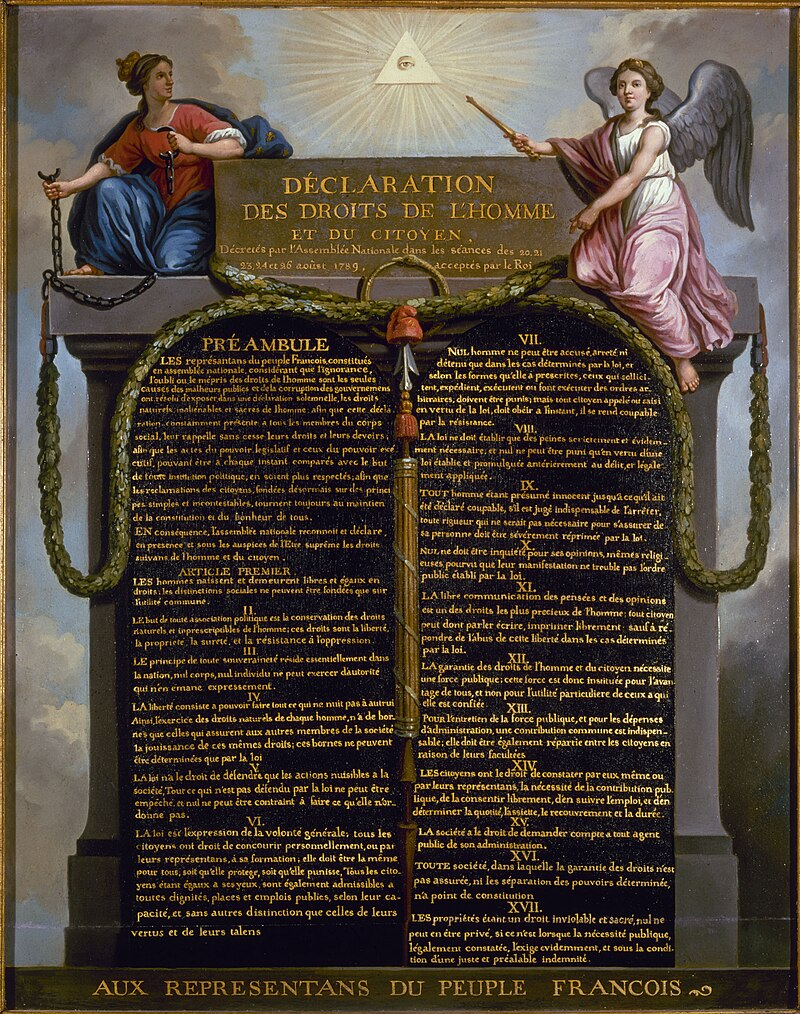
\includegraphics[width=\linewidth]{ddhc}
	\caption{Déclaration des droits de l'homme et du citoyen}
	\label{fig:ddhc}
\end{figure}
Celle-ci comporte un préambule, et si on suit le Conseil Constitutionnel (ce qu'on doit faire), celui-ci fait partie du bloc constitutionnel:
\begin{quote}
	Les représentants du peuple français, constitués en Assemblée nationale, considérant que l'ignorance, l'oubli ou le mépris des droits de l'homme sont les seules causes des malheurs publics et de la corruption des gouvernements, ont résolu d'exposer, dans une déclaration solennelle, les droits naturels, inaliénables et sacrés de l'homme, afin que cette déclaration, constamment présente à tous les membres du corps social, leur rappelle sans cesse leurs droits et leurs devoirs ; afin que les actes du pouvoir législatif, et ceux du pouvoir exécutif, pouvant être à chaque instant comparés avec le but de toute institution politique, en soient plus respectés ; afin que les réclamations des citoyens, fondées désormais sur des principes simples et incontestables, tournent toujours au maintien de la Constitution et au bonheur de tous.
\smallskip

En conséquence, l'Assemblée nationale reconnaît et déclare, en présence et sous les auspices de l'Être suprême, les droits suivants de l'homme et du citoyen.
\begin{flushright}
	Préambule de la Déclaration des
\end{flushright}

\end{quote}
Ce préambule est motivé par un \emph{considérant que}, adoptant un style judiciaire qui date déjà du moyen-âge.
Certains textes du 17è et du 18è siècle sont précédés d'un préambule commençant par un \emph{considérant}.
Il y est écrit qu'il doit être possible à tous d'y accéder toujours, qu'il doit être possible de comparer législatif et exécutif à une norme supérieure.
Il y a déjà une idée de hiérarchie des normes.
Il y a aussi une notion de \emph{réclamation} des citoyens qui n'est devenu réalité qu'après l'adjonction en 1971 de ces articles au bloc constitutionnel.
La DDHC comporte certains des articles de loi les plus importants. Particulièrement l'article 5: \og\emph{Tout ce qui n'est pas défendu par la loi ne peut être empêché, et nul ne peut être contraint à faire ce qu'elle n'ordonne pas.}\fg
L'article 6 est l'un des plus utilisés par le Conseil Constitutionnel: la loi est la même pour tous.
Les articles suivants décrivent plus généralement le cadre dans lequel les lois doivent d'inscrire.

\paragraph{Préambule de 1946}
Le préambule de la constitution de 1946 (\ref{constitution46}) comporte, sans le mentionner directement, des références à la barbarie nazie et à la nécessité de préserver la dignité humaine.
\begin{quote}
	 Au lendemain de la victoire remportée par les peuples libres sur les régimes qui ont tenté d'asservir et de dégrader la personne humaine, le peuple français proclame à nouveau que tout être humain, sans distinction de race, de religion ni de croyance, possède des droits inaliénables et sacrés. Il réaffirme solennellement les droits et libertés de l'homme et du citoyen consacrés par la Déclaration des droits de 1789 et les principes fondamentaux reconnus par les lois de la République.
\end{quote}
On appelle PFRR les \emph{principes fondamentamentaux reconnus par les loi de la République}.
Le préambule ajoute quelques droits récemment acquis pour certaines parties de la société: le droit de vote des femmes, le droit de grève, la collectivisation d'entreprises privées rendant service public.
Le Conseil d'État avait déjà décidé que le préambule de 1946 n'avait pas juste une valeur programmatique mais une valeur juridique.
Par rapport à la grève, l'arrêt Dehene confirme le caractère constitutionnel de ce droit individuel qui doit s'organiser dans un caractère collectif.
Il est limité par les lois qui le réglementent. Il y en a toutefois un très faible nombre, notamment sur la grève dans le service public.
Il y a également un texte sur les informations minimales dans les transports publics.
Le Conseil d'État s'alarmaient déjà en 1950 de ce faible nombre de loi: il y a une marge de manoeuvre pour le pouvoir réglementaire d'encadrer le droit de grève.

\paragraph{Charte de l'Environnement}
La Charte de l'Environnement \ref{CharteEnvironnement}, adoptée en 2003, ajoutée à la Constitution en 2004, met en exergue le principe de précaution.

\paragraph{Les Principes Fondamentaux Reconnus par les Lois de la République}
Cette formule, créée par le Conseil Constitutionnel après 1971, décrit un nombre de principes précisés dans des lois antérieures à la Vème République sous un régime républicain auxquels il décide de donner une valeur constitutionnelle.
\begin{description}
	\item[\emph{Liberté d'Association}] Celle-ci était menacée sous le gouvernement Marcellin après 1968 par une loi qui visait à faciliter la dissolution d'une association.
		Le Conseil Constitutionnel a rendu constitutionnel l'article 1 de la loi du 1er juillet 1901 relative au contrat d'association.
		Celle-ci crée trois types d'associations, celles sans autorisation, celles déclarées et celles reconnues d'utilité publique.
		Un arrêt du Conseil d'État (CE 1956 Amicale des Annamites de Paris) concernant une association étrangère (d'indochinois) soumise à des restrictions car étrangère avait réduit ces restrictions.
	\item[\emph{Droits de la Défense}] Un arrêt du CC de 1976 a entériné ce principe qui n'était pas particulièrement remis en cause.
		Le CC n'avait pas cité de texte pour ce PFRLR.
	\item[\emph{Liberté de l'Enseignement}] Le CC a été saisi en 1977 par des parlementaires de gauche contre une loi jugée trop favorable à l'enseignement privée.
		Le CC valide cette loi mais en profite pour préciser la Liberté de l'Enseignement comme PFRLR.
		La Loi Guizot (sous la Monarchie de Juillet, 1833), la Loi Falloux (15 mars 1850) et la loi Laboulaye (12 juillet 1875).
		Le CC a alors cité une loi budgétaire de 1831 pour élever le principe au rang de PFRLR.
	\item[\emph{Indépendance de la juridiction administrative}] Élevée par une décision du CC de 1980.
	\item[\emph{Idépendance des professeurs d'université}] Le CC a affirmé ce principe par une décision de 1984, suite à la procédure de juger des professeurs par des externes.
		Ce principe a été étendu par la jurisprudence administrative mais aussi constitutionnelle aux maîtres de conférence.
		Il a toutefois été nuancé (et non aboli) à l'occasion d'une QPC de 2010 née après la loi Pécresse sur les responsabilités des universités.
		Ses décrets d'application et notamment le fait que depuis cette loi les professeurs de l'enseignement supérieur répondent à leur chef·fes d'établissement.
	\item[\emph{Compétence des juridictions administratives}] Décision de 1987 définissant le noyau dur de la compétence des JA.
	\item[\emph{Autorité judiciaire garante de la propriété privée}] Loi pour des expropriations massives pour la construction d'une ligne de TGV contestée, le CC a statué sur le fait que la propriété est la compétance du juge judiciaire.
	\item[\emph{Extradition interdite dans un but politique}] Le Conseil d'État (CE 1996 Koné) a statué sur le cas de M. Koné qui souhaitait faire annuler le décret de son extradition.
		M. Koné était poursuivi au Mali (officiellement pour des crimes et délits de droit commun) argait que ses poursuites étaient liées à son statut d'opposant politique.
		La France a adopté en 1927 une loi refusant l'extradition de ses propres ressortissants et celle pour motifs politiques, même accusés d'actions violentes.
		Le Mali réclamait l'extradition non pas pour un crime politique mais pour un crime de droit commun, M. Koné demandait donc que l'extradition soit interdite dans un but politique.
		Le Conseil d'État a donc élevé ce principe au rang de PFRLR au dessus des traités.
		Cependant, le CE a rejeté la demande de M. Koné, jugeant que le PFRLR ne s'appliquait pas dans ce cas.
		La procédure d'extradition se terminant par un décret du PR, si celui-ci venait à refuser de signer le conseil, comme c'est arrivé sous Mitterrand, l'extradition n'aurait pas lieu.
	\item[\emph{Justice pénale des mineurs}] En 2002, le CC reconnaît dans les PFRLR des dispositions particulières pour la justice pénale des mineurs.
		Au minimum, elle signifie que les mineurs ne doivent pas être traités comme des majeurs.
	\item[\emph{Spécificité du droit d'Alsace-Moselle}] En 2011 (le dernier principe consacré), le CC dans une QPC a noté une spécificité du droit en Alsace-Moselle
\end{description}
Il ne faut pas se polariser sur le nombre de PFRLR ni leurs qualifications exactes.
Depuis les années 2000, il y a raréfaction du nombre de caractérisation.
Pour être un PFRLR, il faut qu'il y ait une ou plusieurs lois républicaines antérieures à la IVème, dont le principe est gardé dans la continuité.

\paragraph{Principes et Objectifs Constitutionnels}
Il faut ajouter à ceci les principes constitutionnels tirés des textes liés au préambule (lecture entre les lignes).
Ce sont des règles qui ont la même valeur que les règles explicites.
Il faut également y ajouter les objectifs à valeur constitutionnelle, qui ont une valeur moindre, mais qui servent à soutenir des lois du parlement (droit à un logement décent, accès au droit\ldots).
Dans le cas ou un objectif entre en conflit avec une règle ou un principe, l'objectif est restreint.

\subsubsection{Les Normes Internationales}
L'article 55 de la constitution donne aux traités ou accords régulièrement ratifiés ou approuvés une autorité supérieure à celle des lois.
Suite à la DC de 1975 sur l'IVG, la Cour de cassation (Ch. Mixte, 24 mai 1975, \emph{Cafés Jacques Vabre}) puis le Conseil d'État ont dit que l'article 55 permet au juge de ne pas appliquer une loi française contraire au traité, quelque soit l'ordre de publication des lois.
Dans l'arrêt Nicolo (20 octobre 1989), dans une disposition pour l'élection au parlement européen, le Conseil d'État applique le traité de Rome.
Le contrôle de conventionnalité donne un très grand pouvoir au juge.
La jurisprudence (arrêt Koné; CE 1993 \emph{Sarran et Levacher} sur le système électoral en nouvelle calédonie; Cass. Ass. plén 2 juin 2000) refuse toutefois le principe de la supériorité des normes internationales par rapport à la constitution.
L'article 55 reste cependant flou et la jurisprudence (CE 1999\emph{Groupement de défense des proteurs de titres russes sur le principe d'égalité}) reste souvent nuancée.

\subsubsection{Les Normes Législatives}
Il faut revenir aux articles 34 et 37 de la constitution \ref{constitution}, qui limitent une liste exhaustive et prédéterminée des compétences du parlement.
La loi fixe les règles pour la nationalité, l'état des personnes, sur les crimes et les délits (partie législative du code pénale), l'assiette des impôts, la loi de finance et les catégories d'établissements publics.
Il est dit aussi que la loi fixe les principes fondamentaux dans divers domaines, la propriété, l'enseignement, la défense nationale, le droit du travail\ldots
Les principes fondamentaux ne se réduise pas, comme on pourrait le penser, à quelques règles.
Ceci est destiné à brider les compétences du parlement.
Toutefois, il ne s'agit pas d'une compétence qui est retirable au parlement.
Le respect de cet article 34 est contrôlé par deux mécanismes qui doivent permettre au gouvernement d'éviter que le parlement n'aille sur le domaine réglementaire: l'article 41 spécifie qu'au cours de la discussion d'une loi et de la proposition d'amendement, le gouvernement peut proposer une exception d'inconstitutionnalité, mais c'est très rare.
Le gouvernement a même toléré que le parlement déborde de l'article 34 sur des projets de loi.
Le deuxième mécanisme, le deuxième alinéa de l'article 37 permet de faire appliquer cette règle rétroactivement.

Les normes législatives regroupent l'ensemble des lois ordinaires (cf supra sur l'article 34), les lois organiques (article 46), les ordonnances (ancien article 92, article 38 si ratifiées, sinon elles gardent le statut d'acte administratif) et des mesures de l'article 16 (CE 1962, \emph{Rubin de Servens}, donne le pouvoir au PR de prendre des mesures sur le domaine législatif).
L'ordonnance est un acte administratif avant la ratification, mais devient une loi après.

\subsubsection{Principes Généraux du Droit}
Les PGD sont des normes jurisprudentielles créées par le Conseil d'État sans leur donner le statut de loi.
Ils sont utilisés pour faire annuler des actes qui iraient à l'encontre de ces principes (Roubau).
\begin{description}
	\item[Droits de la Défense] CE 1945 \emph{Aramu} sur un fonctionnaire de Vichy collaborationniste.
	\item[Droit au Recours] CE 1950 \emph{Lamotte} sur un conflit né pendant le régime de Vichy d'une dame propriétaire d'une terre non cultivée.
		Le régime, vu les difficultés de ravitaillement, a autorisé les préfet a réquisitionner des terres non cultivées.
		La loi de 1943 décide que les décisions dans ce domaine sont sans recours administratif.
		Le CE va décider d'annuler l'arrêt.
	\item[Égal Accès aux Emplois Publics] CE 1954 \emph{Barel}, le ministère de l'intérieur refuse que concourrent à l'ÉNA ceux qui sont soupçonnés de proximité avec le Parti Communiste.
		Le CE déboute le ministère.
	\item[Égalité devant les Charges Publiques] CE 1958 \emph{Syndicat des propriétaires de chênes-lièges d'Algérie},
	\item[Développement de la Famille] CE 1978 \emph{Gisti}
	\item[Dignité de la Personne Humaine] CE 1994 \emph{Milhaud} et CE 1995 \emph{Commune de Morsang-sur-Orge} (Lancer de nain)
	\item[Liberté Contractuelle] CE 1998 \emph{Corenette de Saint-Cyr}
	\item[Prescription du Code Civil]
\end{description}
Ils ont une valeur \emph{infra-législative et supra-décrétale} (sauf à se confondre avec les principes constitutionnels comme la continuité des services publics, CC 1979 (décision sur le droit de grève dans l'audiovisuel public)).

\subsubsection{Les Règlements}
On parle ici des règlements dans le sens le plus large: actes administratifs issus du pouvoir réglementaire au sens de l'article 37 de la Constitution.
Les décrets sont faits par le PR ou le PM.
Il y a des décrets individuels émanant du pouvoir réglementaire (admission à un concours, etc\ldots) et des décrets généraux (appelés règlements au sens strict).
Le décret individuel est toujours une application, soit d'une loi, soit d'un décret général.
Le gouvernement détermine la politique de la nation, et est dirigé par le premier ministre.
Les décrets du PR doivent être approuvés en conseil des ministres.
La constitution ne prévoit toutefois pas de répartition des décrets entre PM et PR, exceptés certaines nominations.
Il y a bien plus de décrets du PM que du PR mais ceux ci ont la même valeur.

\medskip

Un ministre ne prend jamais de décrets mais des arrêtés, sur délégation du Premier Ministre, en fonction de leurs compétences.
Le texte de base pour déterminer ces compétences est celui de la formation du gouvernement.
L'arrêt Jamart de 1936 donne aux ministres comme aux directeurs de toute autorité administrative le pouvoir de prendre des règlements.

\subsection{Étude de Décisions}
\subsubsection{CE 3 décembre 1999}
\ref{CE3121999}

\subsubsection{CE 30 octobre 1998}
\ref{CE30101998}

\section{Les Ordres Juridiques Européens}
Il y a un grand déficit d'informations sur les structures juridiques du droit européen.
Ces structures juridiques correspondent à deux ordres différents, celui de l'Union Européenne et celui du Conseil de l'Europe.
Les traités (dans un pays moniste comme la France) et le droit secondaire (traités européens et jurisprudence des deux cours européennes) sont directement intégrés dans le droit français, à une position très élevée dans la hiérarchie des normes.
La moitié des contentieux (environ) mentionnent dans le visa des normes européennes.

\subsection{Le droit de l'Union Européenne}
Le droit primaire (des traités) et le droit dérivé (règlement, décisions) forment le droit de l'Union Européenne.
Le droit dérivé (en partie) ne nécesite pas de ratification, et est intégré dans la droit français au même niveau que les traités,
Les directives quant à elle nécessite un modification.
CECA en 50, Rome en 57. Depuis 1992 et Maastricht quand l'Union Européenne est créée, elle a été réformée Amsterdam 1991, Nice 2001 (2003 pour la ratification).
Après l'échec du projet de constitution européenne, le traité de Lisbonne est le dernier mis en place.
Depuis Maastricht, il y a deux traités, le plus court, celui de l'UE (le TUE) et le traité de fonctionnement de l'UE (TFUE).

\smallskip

Le TUE donne à l'UE son cadre institutionnel avec ses conseils (Conseil avec un Président élu, Commission, Parlement, CJUE).

Le conseil de l'UE peut correspondre à plusieurs institutions, par exemple le conseil des ministres de l'UE (où chaque état est représenté par un ministre compétent).
La présidence du conseil tourne entre les divers gouvernements tous les 6 mois (actuellement la Hongrie).
Ce conseil participe et a une grande part au pouvoir législatif.
Il a rôle dans la formation des règlements et des directives, avant qu'elles passent par la commission.
Il peut y avoir des processus de co-décision avec le parlement.
Il y a des procédures de vote complexes (pondération selon le nombre de voix par état, diverses majorités).
L'autre conseil, plus connu médiatiquement, est le conseil européen, qui se tient au minimum deux fois par an.
C'est le conseil des chefs d'état et de gouvernement (le PR en France), qui est doté d'un président permanent (actuellement Charles Michel, homme politique belge).

La commission Européenne est un organe très important avec un pouvoir exécutif et d'initiative.
Toute norme européenne doit passer par la commission.
Chaque état a droit à un membre, elle prend des décisions individuelles.
Le parlement siège à Strasbourg et à Bruxelles, la commissions à Bruxelles et le CJUE à Luxembourg.

Le TFUE résulte d'une superposition de normes, qui reprend l'acquis communautaire (libre circulation, politique agricole commune\ldots) et y a ajouté les deuxièmes et troisièmes piliers: politique commune étrangère et de sécurité (gérée par un Haut Représentant, M.Borel), et les affaires politiques communes pour créer un espace de liberté, de sécurité et de justice.
Depuis le traité de Nice, on n'utilise plus les expressions deuxièmes et troisièmes piliers.
Il existe une charte des droits fondamentaux de l'UE, qui a supposément même valeur que les traités, mais qui a tout de même une possibilité d'\textit{opting out} qui permet d'en sortir.
Elle répète en majeure partie le contenu du bloc de constitutionnalité.
Elle n'a pas vocation de s'appliquer dans les États, mais plutôt de s'assurer que les droits fondamentaux ne sont pas violés par les institutions et normes européennes, ni par ses agents.

\smallskip

Le droit dérivé est constituté de trois types de normes, les règlements, directives et décisions (normes individuelles concernant des personnes juridiques).
Le projet de constitution européenne proposait d'appeler \emph{lois} les règlements.
Dès que le règlement a été élaboré par la commission, accepté et voter par le conseil des ministres et le parlement, il rentre en application dans le droit français.
Toutes les normes dérivées n'ont pas besoin d'une autorisation de ratification.
À la différence du droit international, le droit européen n'admet aucune excuse de réciprocité.
Aucun état ne peut refuser d'appliquer une norme car un autre état n'applique une norme.
Ce sont des traités qui engagent fortement.
Les directives portent sur des sujets où il existe des normes nationales mais où les organes de l'UE cherchent à uniformiser.
Ces directives doivent être transposées dans le domaine national (cf. articles 34 et 37 de la constitution \ref{constitution}).
Chaque directive fixe un délai de transposition.

\smallskip

La Cour de Luxembourg (CJUE) a un juge par état, accompagnés d'avocats généraux (au même sens qu'à la CCass).
Quand on parle de la Cour, on parle aussi du tribunal de première instance qui juge les questions relatives à la fonction publique européenne (il y a eu un tribunal spécifique de 2004 à 2016) mais aussi les recours des personnes morales contre les décisions de la commission, essentiellement en matière de concurrence.
La Cour juge différents types de recours: en annulation, en carence, en réparation, en manquement et répond aux questions préjudicielles en interprétation des traités.
Tout juge peut, lorsqu'il a un doute sur une norme européenne, entamer une procédure de question préjudiciaire.

La jurisprudence européenne se base déjà sur les grands arrêts sur la primauté du droit communautaire.
En se basant sur des arrêts (\textit{Van Gend en Loos} (1963), \textit{Costa c. Enel} (1964), \textit{Simmenthal} (1978 sur les lois postérieures)), la Cour dit que le droit européen est une forme très originale de droit international.
La Cour dit que les normes européennes ont primauté sur les normes nationales, y compris sur les normes postérieures.
Cette primauté n'est pas soudainement apparue dans le projet de constitution européenne, mais existait déjà aux traités de la CECA et dans le traité de Rome.
La Cour répète que c'est le devoir de tout juge national de faire prévaloir le droit européen, y compris sur une loi nationale contraire et postérieure.
On essaie toutefois d'éviter les conflits entre droit constitutionnel et européen.
La CJUE a également reconnu l'effet direct aux directives non transposées dans le délai prescrit (CJCE 1974 \textit{Van Duyn}, 1991 \textit{Francovich} et \textit{Mme Bonifaci}).
La CJUE peut condamner les États et donne aux particuliers la possibilité d'agir en justice contre les États.

\subsection{CEDH}
Le Conseil de l'Europe (qui n'est pas l'UE), remonte à l'après guerre, et s'est étendu au bloc soviétique après 1989.
Il y a actuellement 46 membres, seules la Russie est suspendue et la Biélorussie n'a jamais été admise.
Le Conseil de l'Europe a deux organes (un parlement où il y a des délégués des parlements des états, des réunions des chefs d'états et des ministres).
La CEDH (convention), signée en 1950 à Rome, se présente sous la forme de 17 articles sur les droits à garantir et la procédure à suivre pour faire respecter ces droits.
La CEDH n'a été ratifiée par la France qu'en 1974 sous l'intérim du président Poer et en
Il y a aussi des protocoles supplémentaires sur le contrôle du droit de propriété par exemple.
Jusqu'en 1994, les recours présentés devant la Cour Européenne des Droits de l'Homme de Strasbourg.
La procédure s'est simplifiée.
Pour accéder à la Cour de Strasbourg, il faut avoir épuisé toutes les voies de recours internes.
La Cour de Strasbourg rejette 99\% des recours, par un processus institué par le protocole 14 permettant d'écarter les requêtes manifestement infondées.
Les recours se font d'une personne contre un État, dans lequel la personne réside ou dont la personne a la nationalité.
Elle siège toujours dans la composition suivante: le juge d'où vient la plainte qui juge en toute indépendance, et 16 autres juges.
La cour met en avant des affaires dans des arrêts \textit{pilotes}, en supposant que les juridictions nationales pourront faire leur travail après.
La Cour influe fortement sur les pratiques, par exemple, la France a été condamné pour des violences faites dans les commissariats (Tomazi 92, Rivas 2004).

\smallskip

La jurisprudence de la Cour de Strasbourg est une jurisprudence particulièrement évolutive.
Le principe même, dès l'origine, est que les états membres du Conseil de l'Europe qui ont adhérés à la CEDH ne sont pas parmi les pires dictatures au monde et respectent les droits de l'Homme a un niveau satisfaisant.
La Cour, quand elle constate une violation, condamne, et se montre de plus en plus exigente à travers le temps.
La Cour dit aussi que les termes ne doivent pas être interprétés dans chaque état, mais tous selon une interprétation commune dictée par la cour.
Par exemple, la procédure d'emprisonnement est considérée comme du pénal par la cour, mais pas dans certaines législations.
La Cour laisse toutefois aux États une marge nationale d'appréciation. Elle a admis et admet encore que la législation sur l'avortement soit différente dans tous les états.

\subsection{Effets sur la Jurisprudence Administrative}
Historiquement, le CE était souverainiste et réticent à l'égard du recours préjudiciel.
Le CE, lorsqu'il y avait un doute sur l'interprétation d'un traité envoyait au ministère des affaires étrangères.
Désormais, le CE est celui qui fait le recours à la question préjudicielle, et tient compte de l'avis de la CJUE.
À ce contrôle de conventionnalité (qui se greffe sur le recours pour excès de pouvoir).
Par l'exception d'illégalité, on écarte la norme législative, la norme réglementaire peut être annulée.
C'est au conseil des ministres de vérifier les nouveaux traités pour aménager le droit français.
Il arrive toutefois qu'il y ait des divergences avec la jurisprudence de Strasbourg.
Il y en a très peu, mais, qu'il le veuille ou non, le CE finit par s'incliner.

\subsection{Étude de Décisions}
\subsubsection{Décision du Conseil d'État du 7 février 2003 \textit{Gists}}
\ref{CE7022003}

Il existe plusieurs types de contrôle possibles:
\begin{description}
	\item[Le Contrôle Minimum] qui agit sur le pouvoir décisionnaire
	\item[Le Contrôle Restreint] qui agit devant les erreurs manifestes d'appréciations
	\item[Le Contrôle Normal] qui agit sur les erreurs de droit
	\item[Le Contrôle Renforcé] qui agit en cas de non-respect de la proportionnalité. C'est notamment le cas des actes sur avis conforme.
\end{description}

\subsubsection{Décision du Conseil d'État du 2 février 2024}
\ref{CE2022024}


\section{La Notion et les Caractères du Service Public}
\subsection{Définition de Service Public}
Le terme \emph{service public} désigne l'ensemble des administrations et entreprises qui gèrent des concepts liés à l'organisation.
On y distingue les compétences dites \emph{régaliennes} de l'état
CCons 1986 sur les privatisations désigne par attributions régaliennes la police, la justice, les finances et la défense nationale des attributions qu'elle ne peut pas déléguer à des personnes privés.
Historiquement, elles l'ont partiellement été, avec la Ferme Générale sous l'Ancien Régime.
Par les Partenariats Publics Privés (PPP), le privé est associé à la construction et la gestion de prisons.
Historiquement, le premier service public est la Poste (créé par Louis XI), mais elle n'a plus le monopole de ce service, ce qui crée un système de concurrence.
Le terme service public a été employé dans des actes administratifs, et notamment du CE, jouant un rôle important dans la jurisprudence et la doctrine administrativiste autour des 19è et 20è siècles.

La décision du tribunal des conflits Blanco (1873), concerne la mutilation d'une petite fille renversée par un wagonnet mal contrôlé par un ouvrier de la manufacture d'État des tabacs.
Son père a agit en justice au civil pour demander une indemnité, et le préfet a élevé le conflit au tribunal des conflits (tout juste rétabli par une loi de 1872).
L'arrêt considère que, puisqu'il s'agit de personnes employées par l'état, d'ouvriers de l'état (pas de fonctionnaires de l'état), il s'agit bien de la compétence administrative.
Le CE a rendu ensuite un arrêt qui accorde au père, pour sa fille, une rente d'invalidité à vie.
Plusieurs auteurs (notamment Léon Duguit, Jèze, Bonnard, Rolland), ont mis cet arrêt en avant pour concevoir l'état comme un ensemble de services publics.

\medskip

L'arrêt du CE \emph{Terrier} de 1903, concerne l'inquiétude du Conseil Général de Saône et Loire sur la prolifération des vipères.
Le CG propose une prime à ceux qui rapporteraient des vipères mortes, et le dénommé Terrier n'a pas été payé ce qu'il attendait en rapportant des vipères.
Le CE décide que le contrat définit un service public dit \emph{matériel ou fonctionnel} plutôt qu'organique, sans bureau ou fonctionnaire, délégué à des personnes privées.
De manière similaire, la jurisprudence a été appliquée pour l'arrêt CE 1961 \emph{Magnier} sur les hannetons.

On définit alors un service public une activité d'intérêt général pris en charge par la personne publique (cas de \emph{régie}, on dit que le service publique est \emph{assuré}), ou délégué à une personne privée (on dit que le service est \emph{assumé}).

Les services publics ont formé une notion centrale en droit administratif jusqu'à la crise des services publics annoncée dans les années 1970 et 1980 (on en parle toujours).

Les personnes morales s'opposent aux personnes physiques.
Parmi les personnes morales, certaines sont de droits privé (associations et entreprises), et d'autres sont de droit public (parmi lesquelles l'État et les Collectivités Territoriales notamment).
Les personnes publiques se distinguent des personnes morales privées par leur mode de création (des lois ou des règlements au lieu de contrats volontaires par lesquelles des personnes s'associent),
par l'absence de liberté d'adhésion (personne n'est forcé d'entrer dans une société ou une association, mais nous sommes rattachés (pour partie involontairement et pour partie volontairement) à une état par la nationalité ou la résidence sur le territoire, à une collectivité territoriale par le lieu de résidence, à des établissements publics par davantage de choix (on choisit de se présenter au concours de l'ENS par exemple))
et par des prérogatives de puissance publique ().
Les personnes physiques correspondent à des êtres humains, mais la personne physique du droit est une abstraction, comme tout concept juridique, c'est une conception de l'esprit qui réduit et en même temps dignifie chacun en une personne juridique, mais une personne juridique unique.
On peut difficilement dire que l'État est créé par la loi, mais c'est une construction juridique.
L'État moderne se confond à l'ordre juridique national. Pour un juriste, l'État n'est pas l'appareil d'État, mais c'est l'ensemble des normes qui constituent l'ordre juridique.
Sur Gallica, on trouve un article de Kelsen de 1926 dans la Revue de Droit Public, où il explique d'abord qu'il fait la différence entre l'état au sens des normes et l'état personne morale (personnification juridique nécessaire, apparue tardivement) au sens de l'ensemble de ses agents.

\subsection{Les Services Publics}
L'état, en tant que personne morale, unifie les administrations, les collectivités territoriales (communes, départements et régions depuis 1982) et des établissements publics (distingués à partir de 1862 des établissements d'utilité publique).
Les établissements d'utilité publique sont des associations (personnes morales de droit privé, créées par un contrat) qui ont été reconnues par un processus passant par le conseil d'État.
Ceci leur permet de recevoir des délégations de services publics, mais ce n'est pas nécessaire.
Les établissements publics, quant à eux, sont nationaux ou non, et comportent par exemple les universités, les établissements de coopération intercommunale, etc\ldots
Historiquement, les établissements publics nationaux sont appelés des démembrements de l'État. Les facultés n'avaient pas la personnalité morale avant la 3ème République, et ont été regroupée par la loi de 1896 sous des universités qui elles, ont la personnalité morale.
Les UMR sont des démembrements des universités et du CNRS et n'ont pas la personnalité morale.
Les collectivités territoriales peuvent créer des établissements publics (régionaux, départementaux, communaux) et des établissements de coopération intercommunale, établissements publics formés entre commune.
Par exemple, les syndicats de commune pour mettre en commun un ou plusieurs services publics (Syndicat Intercommunal à Vocation Unique (SIVU) et Syndicat Intercommunal à VOcations Multiples (SIVOM)), notamment pour les SICTOM.
Le CGCT (Code Général des Collectiités Territoriales) régit tout ceci.
Les établissements publics se voient attribués un domaine de l'état.
Foljuif est un leg d'une personne à l'École Normale Supérieure. On appelle ceci un domaine privé dont la gestion relève pour l'essentiel du droit privé.
Il existe des formes plus générales de gestion privée des services publics.
Tout ce que fait l'état ne relève donc pas nécessairement de l'ordre administratif.
Parmi les établissements publics, on distingue les EPAdministratif (hôpitaux à but social), les universités (ESPC), le CNRS (ESPT), les grandes écoles (dont l'ENS, EPSCP) ou les musées (à caractère culturel).
Dans l'arrêt TC 1921 \emph{Bac d'Eloka}, le tribunal des conflits considère qu'un service public qui gère un établissement à caractère commercial (ici, un bac maritime pour traverser un lac dans une colonie) est sous l'autorité judiciaire.
Les établissements à but industriel et commercial (EPIC) sont soumis à trois critères cumulatifs: avoir un objectif industriel et commercial du service, avoir des ressources propres financées par les usagers et avoir un mode de fonctionnement comparable au privé (un EPIC doît être rentable).
Depuis les privatisations (Jospin\ldots) les EPIC sont réduits en nombre, limités à la RATP, l'Opéra, la RMN, le CEA et le CNES.
La SNCF a connu trois statuts différents qui interviennent beaucoup dans les arrêts.
De 1937 (la nationalisation) à 1982 la SNCF est une société anonyme de droit privé. L'État a simplement pris 100\% du capital.
De 1982 à 2020, la SNCF était un EPIC. Les cheminots de la SNCF sont principalement des agents de droits privés.
Seuls le président/DG et le comptable public sont obligatoirement des fonctionnaires.
En 2020, la SNCF a été retransformée en société anonyme de droit privé.

Il existe des situations où un EPA gère ce qu'on appelle un SPIC (Service Public Industriel et Commercial) et réciproquement des EPIC gèrent des SPA (Service Public Administratif).
Par exemple, les chambres de commerces (EPA) gèrent les ports maritimes. L'ONF est un EPIC qui gère la conservation du patrimoine et l'accès au public (SPA).
Jusqu'aux années 1990, la Poste (PTT) était une administration d'état. Lorsque Poste et France Télécom ont été séparés, la Poste n'a pas été privatisée mais est devenue une société anonyme (personne morale de droit privée) à capitaux publics.
Il existe des associations syndicales de propriétaires (en milieu rural, associations qui incitent fortement les propriétaires à participer à des opérations de drainage, de protection des forêts ou des dunes par exemple).
Dans une affaire remontée au TC en 1889 \emph{Association Syndicale du Canal de Gignac}, le TC a dit que les ASP étaient des établissements publics.
Quant à elle, la Banque de France est une personne morale de droit public qui n'est ni l'État ni une collectivité territoriale, ni un établissement public.

Les missions de service public peuvent être confiées à des personnes de droit privé (CE 1942 \emph{Monpeurt} et 1943 \emph{Bouguen}),
par exemple, toutes les fédérations sportives agréées (qui dépendent d'un comité olympique et même plus), les Associations Communales de Chasse.
Si la CAF et la CNAM sont des EPA, les caisses primaires sont des personnes morales de droit privé.

On parle de lois du service public (parfois lois de Rolland) pour désigner des jurisprudences du Conseil d'État élevées par le Conseil Constitutionnel.
Le service public est soumis à trois principes.
Le principe de continuité (notamment dans la jurisprudence relative aux délégations de service public) précise que le service public ne doit s'arrêter complètement par moments.
Sur l'ORTF il y a par exemple un service minimum.
Le principe d'adaptabilité du service public, moins avantageux pour les usagers, doit s'adapter aux besoins du public (le CE dit qu'une ligne de tramway doit s'adapter aux mouvements de population) mais aussi aux besoins du service public (CE 1948 \emph{Société l'Aurore} sur les prix de l'électricité qui augmentent).
Le principe d'égalité devant les services publics (adaptation du principe constitutionnel d'égalité, article 6 de la DDHC) proscrit toute discrimination injustifiée.
Toute la difficulté est de déterminer la notion de situation semblable.
Exemple célèbre des deux visions du principe d'égalité (CCons et CE), l'arrêt CE 1974 \emph{Denoyez et Chorques} sur le bac de l'Île de Ré, portant sur le nouveau tarif du bac distinguant les habitants de l'île (tarif minimal), les habitants du continent (tarif le plus élevé) et un tarif intermédiaire pour les habitants de la Charente-Maritime, annule la délibération du Conseil Général en considérant que le tarif intermédiaire est une atteinte au principe d'égalité.
Il est considéré que l'administration ne peut pas créer ça, et le parlement vote, en 1979, une loi reprenant le tarif à trois niveaux.
Cette loi, soumise au CCons est validée.
Cela peut paraître contradictoire, mais le parlement peut créer, pour des motifs d'intérêt général dont il est le juge souverain, des discriminations.
Toutefois, cela ne signifie pas que l'administration en a le droit.
Il y a nombre de jurisprudences sur ce principe.

À ces principes majeurs, on pourrait ajouter le contenu du CGFP (Code Général de la Fonction Publique) et notamment les articles L121-1 et L121-2 qui définissent les devoirs du fonctionnaire en quatre mots: dignité, impartialité, probité, intégrité.
Le principe de neutralité du service public (notamment renforcé à l'article L121-2 par la neutralité religieuse) est un principe fondamental aussi, bien que moins important.
Le principe de laïcité (très spécifique à la France) est, pour les fonctionnaires, une déclinaison du principe de neutralité.

L'organisation du service public de la justice relève du droit public de la justice relève du droit administratif.

\section{Les Décisions Administratives et leurs Modifications}
\subsection{Les Différentes Décisions Administratives}
La très grande majorité des décisions administratives est régie par les règles du droit administratif, mais pas toutes. Notamment en ce qui concerne la gestion du domaine privé.
Ici, on parle des actes de l'administration soumis a droit administratif au sens le plus étroit, et on ne parle pas de contrats qui lient l'administration à un prestataire, puisque étant des actes bilatéraux, ils ne sont pas soumis aux recours pour excès de pouvoir mais au plein contentieux.
On ne s'intéresse ici qu'aux actes unilatéraux, que l'on sépare entre actes réglementaires, actes individuels et décisions d'espèce.
Les actes réglementaires ont une portée générale (souvent l'ensemble de la population, parfois pour des catégories de personnes).
Dans un acte réglementaire, a priori, on ne nomme pas une personne.
Les actes individuels, a contrario, concernent des personnes dénommées.
Ils peuvent s'adresser à une seule personne comme à un collectif, dès lors que les personnes sont dénommées.
Les actes réglementaires et individuels émanent tous les deux du pouvoir réglementaire (le pouvoir d'édicter des normes, le PR et le PM par leurs décrets, les ministres par l'autorité qui leur est déléguée\footnote{ils n'ont pas de pouvoir propre}, les actes préfectoraux\ldots).

La question de la délégation de compétence ou de pouvoir introduit une nuance (avec une solution claire bien que contre-intuitive).
Quand est formé un cabinet ministériel, le premier ministre (qui est seul détenteur d'un pouvoir réglementaire primaire) délègue son pouvoir aux ministres dans un décret qui va déterminer les compétences de chaque ministère.
À chaque gouvernement, il y a des changements de portefeuille, des changements de noms\footnote{Qui ne sont pas un exemple de bonne dépense des deniers publics}, il y a un arrêté qui va préciser que le PM se déssaisit d'une partie de son pouvoir.
Il y a le même mécanisme dans toutes les communes dans la désignation des adjoints au maire.
Ces délégations de pouvoir ou de compétence sont des actes réglementaires, même quand peuvent y figurer les noms des personnes qui y sont désignés.
Ces actes, parce qu'ils concernent la répartition des compétences du service public avec vocation à durer, sont considérer ainsi par la jurisprudence. Si il y a changement de ministre sans changement de compétence, il n'y a pas besoin de refaire l'arrêt.
Un autre procédé, est la délégation de signature. Tous les actes qui émanent d'un ministère ne sont pas signés par le ministre.
Le ministre va donc déléguer sa signature à des chefs de service.
La délégation de signature est nominative, et n'est pas à une fonction comme la délégation de compétence.
Cela ne signifie pas que le délégant se dessaisit de sa compétence.
La délégation de signature est un acte individuel dont les effets sont moins important que la délégation de pouvoir.

Les décisions d'espèce sont apparues dans la jurisprudence, notamment dans CE 1974 \emph{Adam} sur la déclaration d'utilité publique pour le tracé d'une autoroute. Le CE a décidé qu'on était en présence d'une décision susceptible au recours pour excès de pouvoir qui n'est ni réglementaire ni individuelle.
Elles arrivent par exemple pour des travaux publics nécessitant un grand nombre d'expropriation, il faut (en respect de l'article 17) une loi/un acte réglementaire prévoyant les travaux sans rentrer dans le détail, suite à laquelle il y a une déclaration d'utilité publique qui prévoit un tracé et une discussion, puis des actes d'expropriation (qui sont des actes individuels).
L'acte intermédiaire ici est appelé une décision d'espèce.
Selon le type de décision, les décisions d'espèce vont être tantôt jugé comme un acte réglementaire ou un acte individuel.
Un autre exemple typique de décision d'espèce est la convocation d'électeurs à un vote. Dans un cadre législatif ou réglementaire prévoyant quand faire des élections, il y a des décrets organisant les élections et convoquant les électeurs.
Une première conséquence de cette distinction, est que les actes réglementaires et les décisions d'espèces ont seulement des effets de droit (les administrés ont droit à leur application, et sont obligés de leur obéïr) tandis que les actes individuels peuvent créer un droit subjectif (personnel et acquis).
En particulier, il n'y a aucun droit à s'opposer à une modification d'un acte.
Le seul droit est celui à l'application de ces actes et à leur respect, en particulier par l'administration. Elle n'a pas le droit de laisser dormir des textes réglementaires sans les violer mais sans les appliquer.

Du côté des actes individuels, il y a des actes qui ne sont pas créateurs de droit (notamment les mesures de police qui sont des autorisations pouvant être retirées facilement), et d'autres qui sont créateurs de droits acquis.
Cela ne signifie pas droits éternels.
En particulier, un fonctionnaire ne peut être privé de son droit et de son emploi (en particulier du traitement afférent) que par une procédure disciplinaire.
Tous les permis (de conduire, de construire\ldots) sont des actes individuels.

Tous ces actes font objets du recours pour excès de pouvoir.
Au cours des 19 et 20è siècles, pour être soumis à un recours, la justice administrative demande qu'un acte soit décisoire qui doit modifier (ou maintenir\footnote{C'est une manière de progresser}) l'ordre juridique.
Pendant longtemps, le juge administratif et la doctrine administrative disait que l'acte administratif faisait \emph{grief} au requérant.
Ce terme n'est cependant plus utilisé.
Le requérant ne cherchant rarement à agir en soldat de la légalité mais plutôt dans son propre intérêt, on comprend tout de même la notion.

S'agissant des circulaires, une distinction a été faite entre l'arrêt CE 1954 \emph{Notre Dame du Kreisker} et l'arrêt CE 2002 \emph{Mme Duvignères}.
Les circulaires sont une pratique ancienne mais souvent interne à l'administration.
Dès le 19ème siècle, les ministères (notamment régaliens, et le ministère de la justice particulièrement) adressent à leurs fonctionnaires (dans les services centraux et externes) lorsque paraîssent de nouvelles lois et de nouveaux décrets.
Leur usage s'est encore accru au 20ème siècle.
Dès le 19ème siècle, certaines circulaires sont connues du public car imprimées.
En 1954 a intenté un recours pour excès de pouvoir contre une circulaire qu'il connaissait et qu'il pensait illégale.
Le Conseil d'État a été saisi de la question de l'existence des circulaires comme décisions administratives.
Le CE a distingué deux types deux circulaires. Les circulaires interprétatives qui ne font que lire un texte de loi et l'expliquer, sans rien y ajouter, ne sont pas des décisions.
Les circulaires réglementaires, qui ajoutent quelque chose au texte qu'elles sont censées interpréter, et sont alors des actes décisoires.
Celles-ci sont alors soupçonnées illégales.
Le CE a, rarement mais parfois, requalifié des circulaires en arrêté si elles rentraient dans les compétences du ministre.
Jusqu'à l'arrêt \emph{Mme Duvignères} de 2002, le CE a appliqué cette jurisprudence. Cette solution était critiquable car le régime de la circulaire prédétermine la solution du procès et son statut.
En 2002, à propos d'une circulaire du ministère de la justice sur l'aide judiciaire, le CE a décidé que toutes les circulaires seraient désignées comme impératives et pourraient faire l'objet d'un recours pour excès de pouvoir.
À côté des circulaires, il existe les directives, qui sont des instructions qui circulent dans des services et qui indiquent aux fonctionnaires comment ils doivent traiter des dossiers individuels, de manière légale, dans le respect du principe d'égalité.
Le chef de service donne des directives, qui ne sont pas impératives, mais qui servent d'orientation.
L'administration ne commet pas d'illégalité dans le cas où elle ne suit pas une directive sous réserve de bonne justification.
Ceci est par exemple le cas pour l'admission dans des formations.
Il peut y avoir des directives dans des circulaires, mais c'est plus rare que les directives soient connues des administrés.
Il peut arriver qu'une directive le soit, comme par exemple dans la décision CE 1970 \emph{Crédit Foncier de France}.
Le CE déclare que les directives ne sont pas susceptibles de recours car elles ne sont pas décisoires, mais elles sont opposables.
Auquel cas, le juge administrative s'enquiert de la directive et de son application dans la situation en question.
Ceci a toutefois été simplifié: depuis 2008 toutes les circulaires en vigueur sont publiées sur Légifrance, et toutes les ciruclaires non publiées sur Légifrance, ne sont pas en vigueur.; depuis 2020 par l'arrêt \emph{Gisti}, qui étend les critères de recevabilité à tous les documents ayant des effets notables: s'il y a des effets sur les administrés, c'est contestable.
Depuis cette mesure sur Légifrance, on est passés de 25000 circulaires à 10000 circulaires en vigueur.

Il y a d'autres catégories d'actes qui se situent à la marge et qui échappent jusqu'aujourd'hui au recours pour excès de pouvoir.
D'abord les mesures d'ordre intérieur (CE 1995, \emph{Hardouin} et \emph{Marie}). Jusqu'en 1995: On applique le \emph{Minimis non quorat praetor}: les juges ne s'intéressent pas aux mesures d'ordre intérieur car trop peu intéressantes.
Le premier arrêt concerne la mise aux arrêts d'un militaire et le second d'une mesure disciplinaire intra-prison.
La Cour de Strasbourg a décidé que les mesures disciplinaires (particulièrement à l'intérieur des prisons) rentraient dans le domaine pénal en vertu de l'article 6 sur le procès équitable.
Dans cette optique, le CE a décidé que les mesures disciplinaires ne sont plus des mesures d'ordre intérieur et n'échappent pas au recours pour excès de pouvoir.
Il reste quelques mesures d'ordre intérieur, par exemple l'affectation d'un·e étudiant·e dans un groupe de travaux dirigés, mais leur nombre a beaucoup diminué.
Ensuite, les actes de gouvernement (catégorie résiduelle depuis assez longtemps), qui sont aujourd'hui limités aux actes de relation entre les pouvoirs constitués et ceux touchant aux relations internationales de la France.
Les principaux actes pris par le gouvernement sont tout de même susceptibles de recours pour excès de pouvoir (CE 1907 \emph{Chemin de Fer de L'Est}).
Ce n'était pas le cas au 19ème siècle, où le CE rejetait beaucoup de demandes qui étaient prises pour des motifs politiques.
Dans l'arrêt CE 1875 \emph{Prince Napoléon}, après la privation du grade de général du Prince Napoléon par la 3ème République, le prince conteste et le gouvernement prétend que c'est une décision politique.
Le CE va débouter le prince mais par pour le motif avancé par le gouvernement, prétendant que tout acte administratif pris par le gouvernement est administratif et non politique.
Sous la Vème République, le déclenchement de l'article 16 et certaines décisions prises par le Général sont contestées dans l'arrêt CE 1962 \emph{Rubin de Servens} où le CE dit que le déclenchement de l'article 16 est un acte de gouvernement, et qu'en vertu de l'article 16 le PR étant habilité à prendre des mesures à caractère législatif ces dernières ne sont pas contestables pour excès de pouvoir mais que les actes à caractère réglementaire, même sous l'article 16, le sont.
L'arrêt CE 1975 \emph{Paris de la Bollardière} sur les essais atomiques en Polynésie qui s'accompagnaient de mesure excluant la navigation, y compris dans les eaux internationales, rejette un recours contre ces actes puisqu'il s'agit d'un acte de gouvernement qui touche aux relations internationales.
L'arrêt CE 1998 \emph{Mégret} précise que la mission d'un parlementaire est un acte de gouvernement car il touche aux relations entre le gouvernement et le parlement. Le décret de dissolution de l'assemblée nationale est un acte de gouvernement, non susceptible d'un recours pour excès de pouvoir.
Les arrêts CE 1995 et 2003 \emph{Greenpeace} déboutent ces derniers en reprécisant que les relations internationales sont bien des motifs du gouvernement.
Le CE précise bien dans tous ces arrêts qu'il s'agit d'actes administratifs, qui, en l'état actuel du droit, forment des actes de gouvernement et ne sont pas susceptibles aux recours par excès de pouvoir.

\subsection{Procédure Non-Contentieuse}
C'est la procédure qui détermine la manière de créer et d'écrire des actes.
Pendant longtemps, il n'y a eu que peu de règles concernant la procédure non contentieuse.
Depuis 2015 et le projet de simplification du droit du Président Hollande, il y a eu des changements.
Les actes peuvent être édictés sans formalisme précis. Un acte décisoire peut être écrit, oral, tacite ou implicite.
Il peut y avoir au préalable une consultation facultative ou obligatoire et la nécessité d'un avis conforme.
La loi du 11 Juillet 1979 a rendu obligatoire la motivation des décisions individuelles (pas des actes réglementaires) défavorables concernant les administrés, notamment pour les mesures de polices (restriction des libertés publiques, interdiction de manifestation, de réunion, de visa), les mesures de sanction, autorisation avec sujétions, retrait ou abrogation d'une décision modificative de droits, opposition d'une prescription, refus d'un avantage auquel l'administré a en principe droit\ldots
Dans tous ces cas, il faut un énoncé écrit dans la motivation des considérations de fait et de droit qui amènent à la décision (CE 1981 \emph{Belasri}, L211-5 du Code des Rapports entre le Public et l'Administration (CRPA)).
Cet arrêt rappelle de justifier précisément les décisions.

Les actes réglementaires doivent être publiés ou affichés (c'est notamment le cas des actes des collectivités territoriales et notamment municipaux).
Les actes individuels doivent être notifiés (traditionnellement par un courrier postal).

Sur les mesures de police, la personne doit être informé avant l'édiction pour lui permettre de présenter sa défense, dans le respect du principe du contradictoire.
Un décret de 1983 précise qu'il est possible d'annuler ce temps dans le cas, d'un état d'urgence.
L'arrêt CE 1987 FANE annule un décret de dissolution d'une association d'extrême droite puisque le principe du contradictoire n'a pas été respecté.
La loi DCRA du 12 Avril 2000 étend la procédure du contradictoire dans les 6 domaines de la loi de 1979, étendant de 2 à 4 mois de silence avant décision implicite de rejet.
La règle avant 2013 était que le silence valait rejet, mais désormais vaut acceptation.

La modification des actes réglementaires est facile puisqu'il n'y a pas de droit au maintien.
Elle est même obligatoire et requise en cas de circonstances nouvelles de fait et de droit (CE 1930 \emph{Despujol}).
Le recours pour excès de pouvoir n'est pas possible après deux mois.
Toutefois, il y a une exception d'illégalité perpétuelle permet par la contestation d'un acte individuel d'attaquer un acte réglementaire support, consacrée par le décret du 28 novembre 1983 (considérée comme un principe général du droit par CE 89 \emph{Alitalia}).
En invoquant une circonstance nouvelle, on peut par ailleurs demander la modification d'un acte et attaquer une décision implicite de refus.
L'arrêt CE 1990 \emph{Association Les Verts} sur une décision d'espèce (qui maintenait un découpage électoral des cantons sans prendre en compte de potentiels changement de densité de population) illustre ce principe, malgré le rejet final.
Si on devait prononcer un tel recours pour ce genre d'élection, cela causerait quelques remous.

Il faut distinguer deux types de changements: l'abrogation et le retrait.
L'abrogation, plus fréquente, annule l'arrêt pour l'avenir. Le retrait, plus rare, l'annule de manière rétroactive.
Le retrait est admis, notamment dans le cas d'illégalité.
Toutefois, il faut distinguer ici les actes individuels créateurs de droit ou non.
Pour ceux qui ne créent pas de droit, l'abrogation pour l'avenir est toujours possible, le retrait avec effet rétroactif n'est possible que pour illégalité, sans condition spéciale de délai.
Pour les actes individuels créateurs de droit, c'est bien plus complexe, et jusqu'au CRPA de 2015, il n'y avait pas de cadre législatif.
La jurisprudence du CE remontait à l'arrêt CE 1922 \emph{Dame Cachet}.
L'abrogation et le retrait ne sont possibles que pour illégalité sauf dans deux exceptions: si la loi l'autorise ou si les bénéficiaires sollicitent le retrait.
La question se pose alors du délai de retrait (jusqu'à quand l'administration peut elle réparer ses erreurs).
Dans l'arrêt \emph{Dame Cachet}, le CE dit que le retrait doit intervenir dans le délai du recours pour excès de pouvoir.
Toutefois, s'il n'y a pas de publicité pour les tiers (CE 1966 \emph{Ville de Bagneux}), l'administration ne peut pas retirer sa décision.
De même, l'arrêt CE 2001 Ternon dit que pour des décisions explicites créatrices de droit qui n'ont pas été publiées, le délai maximum du retrait pour illégalité est le délai de 4 mois et pour les décisions implicites selon le CRPA art. L242-1.
Ceci nous amène à une subtilité du droit administratif: comment une décision implicite de rejet peut-elle être créatrice de droit?
L'hypothèse qui est sans doute la plus fréquente et qui a donné lieu à des arrêts est l'autorisation administrative de licenciement pour des employés protégés (par exemple les représentants syndicaux).
Supposons que l'administration refuse explicitement cette autorisation.
L'employeur invoque un recours hiérarchique demandant de modifier ce refus d'autorisation.
Si le ministre ne répond pas, c'est une décision implicite de rejet qui crée des droits pour le salarié qui ne peut être licencié.
L'employeur peut attaquer cette décision implicite de rejet, et l'administration peut retirer sa décision si elle estime que c'est illégal.

\section{La Police Administrative --- 1}
\subsection{Distinction Judiciaire -- Administrative}
Quelques considérations de vocabulaire d'abord.
Le mot police vient du grec (signifiant la cité) et a eu un sens très large d'\emph{administration} qui est un terme apparu au 18ème siècle dans le droit.
La polie était l'ensemble des règles qui servaient à maintenir l'ordre dans un pays civilisé.
En histoire du droit administratif on fait référence à un traité de droit administratif écrit par Delamare en 1705, adjoint au lieutenant de police de Paris (poste créé par Louis XIV).
Delamare était un commissaire de police, qui a rédigé le \emph{Traité de la Police} et qui contient un témoignage par des précisions des règles sur les marchés et dans la rue dans le dernier siècle de l'ancien régime.
Le mot peut être pris en différents sens depuis les temps modernes.
Ici, ce qui nous intéresse, c'est la police en tant que fonction, en tant que but et acte, on ne traitera pas des services de police, du ministère de l'intérieur\ldots
Historiquement, la police de l'état (non municipale) est une création du régime de Vichy.
Il faut compter environ 100000 personnes pour la police d'État, 100000 personnes pour la gendarmerie et environ 20000 à 30000 policiers de la mumu.
Ce qui nous intéresse, c'est donc la mission de service public de la police, et comment elle s'exprime par des actes.
Ce qui est très important, c'est donc de distinguer la police administrative de la police judiciaire.
La seconde dépend des autorités judiciaires et dépend du parquet, elle est intégrée à la procédure pénale.
La police administrative quant à elle dépend de l'administration et s'exprime par des actes.
Ses actes sont donc jugés devant la justice administrative.
La police judiciaire suppose la commission d'une infraction qui va déclencher un minimum d'enquête et déboucher, si l'infraction est constatée et les auteurs sont identifiés par un procès pénal.
La police administrative a une fonction préventive, et est censée agir avant la commission d'infraction. Son but n'est pas d'identifier ni de poursuivre les délinquants.
Son but est de maintenir l'ordre public, principe reconnu constitutionnel par le juge judiciaire.

La police judiciaire repose sur des officiers de police judiciaire (OPJ) et des agents de police judiciaire (APJ).
Sont OPJ les gradés dans la police nationale et la gendarmerie mais par dans la mumu pour l'instant.
Les maires de toute commune (mais pas le maire de Paris) sont OPJ. À Paris, c'est le préfet de police qui est responsable du maintien de l'ordre.
Tous les OPJ sont soumis au procureur de la République par le ressort du TJ dont ils dépendent, comme précisé à l'article 16 du code de procédure pénale.
Ce sont eux qui encadrent les enquêtes, qu'elles soient de flagrance (quand un crime vient d'être commis), ou prélable (qui n'a pas besoin d'être en flagrant délit).
Les pouvoirs des OPJ sont moins importants en cas d'enquête préliminaire.
Les contrôles d'identité (article 78 du code de procédure pénale) sont de trois types principaux: le contrôle dit répressif, qui est particulièrement adapté à la PJ (après la commission d'un infraction), des personnes suspectes ou témoins peuvent être soumises à un contrôle sous le
Les contrôles dit \emph{requis} qui sont ponctuels et requis par le procureur qui souhaite lancer dans une zone une opération systématique d'identité. C'est un contrôle de PJ qui doit être fait sous le contrôle d'un OPJ par un APJ.
Les contrôles \emph{préventifs} qui doivent être ponctuels (donc non systématiques) et motivés par la crainte de la commission d'un délit. Ils ne peuvent être faits au faciès des personnes contrôlées.
Sur cette distinction, il y a une jurisprudence: l'arrêt du CE 1951 \emph{Consorts Baud}.
Le CE saisi suite à un décès dans le cadre d'une opération de PJ s'est déclaré incompétent.
Si c'est une opération de la PJ, c'est le juge judiciaire qui tranche selon les règles de la justice administrative.
Si c'est une opération de la PA, c'est le juge administratif qui tranche selon les règles du plein contentieux.
L'arrêt TC 1951 \emph{Noualek} sur une opération illégale a lui été renvoyé au TA.
L'arrêt TC 1978 \emph{Société \emph{Le Profil}} suite à l'attaque d'un fourgon de transport de fonds accompagné de forces de police qui a fait des dégâts collatéraux renvoie le cas au TA puisqu'il considère que la faute a eu lieu non pas dans la poursuite des malfaiteurs mais dans l'encadrement préalable des convois.

La police administrative n'a pas de définition propre, mais une définition doctrinale, l'ensemble des actions de l'administration qui imposent des restrictions aux libertés publiques ayant pour but de maintenir l'ordre public.

\subsection{Autorités de Police}
Au niveau central, étatique, l'autorité de police est le PM.
La jurisprudence de la 3ème république conférait le pouvoir de police au PR.
Dans les trois lois de 1875, le président du conseil n'est même pas nommé.
Dans l'arrêt CE 1919 \emph{Labonne}, le CE décide que le premier code de la route, étant une décision de police administrative, peut être attaqué comme un décret de police.
Dans l'arrêt CE 1978 \emph{Association dite Comité pour léguer l'esprit de la Résistance}, le CE décide que sous la Vème république, le descendant du PR de la 3ème est le PM.
Le ministre de l'Intérieur a un rôle important mais à ne pas exagérer. C'est le PM seul qui a autorité nationale.
Au niveau des départements et des régions, cette autorité passe au préfet.
Au niveau communal, c'est le maire qui prend les arrêtés de police administrative (article L.2212-2 du code général sur les collectivités territoriales).
Les maires sont notamment responsables des fous divagants, des animaux errants, des marchés\ldots
Ceci est la suite de la tradition du pouvoir communal voulu par les révolutionnaires.
C'est un terreau pour le contentieux administratif, les TA sont très attentifs aux arrêtés municipaux, puisque ce sont souvent eux qui donnent lieu au contentieux.
Seules ces personnes (auxquelles s'ajoutent les directeurs d'établissements publics) sont détenteurs d'autorité de police.

La police générale est celle d'ordre extérieur (dans la rue), ce qui se passe dans les maisons, dans l'espace privé, regarde la police judiciaire.
La police administrative n'a pas à pénétrer dans l'espace privé.
Ce principe a connu certaines atténuations (et certaines jurisprudences célèbres: CE 1997 \emph{Commune d'Arcueil} sur des publicités sur bus/abribus de sites minitel pornographiques qui déboute un arrêt d'interdiction au motif que les atteintes à la moralité sans trouble extérieur ne dépendent pas de la police administrative; CE 1995 \emph{Morsang-sur-Orge} sur l'interdiction du lancer de nain qui valide l'arrêt au motif de la protection de la dignité humaine, même aux dépens de la liberté de commerce).
À côté de cette police générale, il existe des polices spéciales dépendant de certaines autorités: la police des étrangers, la police des gens du voyage (qui existe toujours, et qui a récemment perdu son caractère discriminatoire (Loi de 1912) qui forçait les \emph{nomades} à avoir un carnet anthropologique, un carnet de circulation (à distinguer du livret de circulation)), la police de la chasse, la police des établissements dangereux (les usines par exemple)\ldots
Il se pose alors la question des rapports entre police générale et police spéciale, comme celle des rapports entre les autorités étatiques et locales.
Il existe une règle simple (CE 1902 \emph{Commune de Néris-Les-Bains}), une autorité inférieure ne peut que préciser une règle posée par une autorité supérieure.
L'autorité générale peut (en général, mais pas toujours) pallier l'absence de mesures de polices spéciale (cinéma (un film qui a obtenu le visa, peut être interdit dans une commune par un maire);
téléphonie mobile (les arrêtés des maires qui voulaient réglementer les pylônes de relais de téléphonie mobile ont été annulés)).
Puisqu'elle apportent des limites aux libertés publiques, les mesures de police doivent être légalement nécessaires et peuvent faire l'objet d'un contrôle maximum dit de \emph{proportionnalité}, qui est intervenu sur la liberté de réunion.
Organiser une réunion ne nécessite pas à une autorisation de l'état, mais doit donner lieu dans certains cas à une déclaration.
Depuis l'arrêt CE 1933 \emph{Benjamin}, les juges administratifs montrent une forme de suspicion à l'égard des mesures générales d'interdiction et préfèrent des mesures plus adaptées aux circonstances.

Réglementent la police administrative les deux lois LOPSI de 2002 et 2011, réunie dans le Code de la Sécurité Intérieure de 2012, la loi SILT qui reprend des mesures de l'état d'urgence de 2017 et la loi de Sécurité Globale de 2021.
Celles-ci permettent de mettre en place des MICAS (mesures d'assignation à résidence, sur un territoire qui ne peut être inférieur à une commune.)

Sur la liberté de réunion, la directrice de l'ENS a en 2011 interdit une conférence d'un lecteur pro-palestinien pour craintes de rixes en marge de la conférence.
Le CE a dit que la directrice avait eu raison et qu'en général, les discussions à caractère politique n'avaient pas leur place dans le batiment.
Nombreux autres arrêts font jurisprudence sur les cas de distinction police générale et police spéciale: CE 1984 \emph{Guez} sur les spectacles de rues, CE 1987 \emph{Guyot} sur la fermeture d'une discothèque, CE 1997 \emph{Association des Tibétains de Paris} sur l'interdiction de manifestations contre la venue du Premier Chinois.
Le décret loi de 1935 institue une déclaration préalable des manifestations.
La loi du 10 avril 2019 remplace ce décret-loi et précise ses mesures.
Ces restrictions aux libertés sont soumises au triple test de proportionnalité institué par l'arrêt Benjamin et précisé par DC 2008 et CE 2011 \emph{Association pour la promotion de l'image}.
Une mesure d'interdiction doit être nécessaire (risque important de trouble à l'ordre public), adaptée (premier moyen est de renforcer la sécurité), et proportionnée (peu de choix des moyens).
\textbf{Il est de bon ton, notamment dans les copies de concours administratifs, de citer les propos d'un juriste allemand Fleiner qui commente une décision Kruizer, qui a été reprise par le vice président Sauvet: \emph{On ne tire pas au canon sur des moineaux}}
La jurisprudence CE 1909 \emph{Abbé Olivier} reste le principe pour les manifestations religieuses; et les \textit{raves} ont fait l'objet d'une intervention spécifique de la loi en 2001, désormais intégrée au CSI.

Le juge administratif n'est pas tenu de considérer le contrôle maximum, il peut ainsi passer du contrôle minimum (pouvoir discrétionnaire) à l'erreur manifeste d'appréciation (CE 1973 \emph{Librairie François Maspero}), voire au contrôle maximum des mesures de police.
Le juge peut également sanctionner le détournement de pouvoir, le non-respect du principe d'égalité ou l'abstention illégale (CE 1983 \emph{Veuve Lefebvre}).
Les contraintes pesant sur l'administration sont moindres en vertu de la théorie des circonstances exceptionnelles: CE 1918 \emph{Heyriès} et 1919 \emph{Dames Dol/Laurent} (deux péripatéticiennes du port de Toulon contestent un arrêté du préfet maritime d'interdiction de la prostitution se sont vues débouter).
Les circonstances exceptionnelles, notamment mais pas exclusivement les circonstances de guerre, relâchent le contrôle du juge administratif sur les mesures de police.

Alors qu'on nous explique que la police traditionnellement est limité à l'ordre extérieur et dans la rue et que la projection de film peut entraîner des troubles, l'attribution de visas se fait avec pour but la protection des mineurs par une décision nationale du ministère de la culture sur un avis simple d'une commission étatique.
Cette décision fait l'objet du contrôle normal du juge administratif (CE 1975 \emph{Société Rome-Paris} sur l'interdiction nationale d'une adaptation de \emph{La Religieuse} de Diderot, reconnaît la compétence du JA).
Dans les décennies suivantes, plusieurs affaires du même type ont eu lieu, souvent à l'initiative des producteurs et réalisateurs.
Le CE (CE 2000 \emph{Association Promouvoir}) donne raison à un requérant se plaignant d'une restriction trop limitée portant sur le film \emph{Baise moi} (d. 12 juillet 2001) et annule le visa qui autorisait le film aux mineurs de moins de 16 ans, alors que la jurisprudence prévoit qu'un film qui comporte un grand nombre d'images pornographiques et violentes, qui n'est pas assorti d'un message de prévention et dont le caractère artistique paraît mineur devant ces images doit être interdit aux mineurs de moins de 18 ans.
La même chose est arrivé au film \emph{Love}.
Puisqu'il s'agit d'une décision nationale, celle-ci est toujours présentée au Conseil d'État.
Les membres de la chambre regardent le film et jugent de l'affaire.
Les films classés X font l'objet d'une fiscalité lourde et l'absence d'une diffusion publique.
Il peut être aussi tenu compte dans ce procès national des relations dans un film à caractère policier ou judiciaire à un procès en cours.
L'arrêt CE 1979 \emph{Chabrol Noces Rouges} autorise l'interdiction temporaire d'un film puisque l'affaire relatée dans le film n'avait pas encore été jugée en assises.
À celà s'ajoute la possibilité pour les maires d'utiliser leur pouvoir de police général d'interdire un film s'il y a un risque de troubles matériels ou des circonstances locales.
Pendant quelques décennies, les maires pouvaient faire état d'une sensibilité particulière de la population de leur commune (CE 1959 \emph{Société des films Lutétia de Dijon} à propos des \emph{Liaisons Dangereuses}).
Après avoir donné lieu à des validations dans les années 60, cette jurisprudence s'est plutôt traduite par des annulations (CE 1985 \emph{Ville d'Aix-en-Provence} (à propos du \emph{Pull-over rouge}), TA 1990 Bordeaux \emph{Commune d'Arcachon} (à propos de \emph{La dernière tentation du Christ} dont le visa avait été confirmé par CE 1990 \emph{Pichène}))
\section{La Police Administrative --- 2: La Police des Étrangers}
Peu de dispositions s'appliquaient aux 19e siècle aux mesures d'élgoignements du territoire des étrangers.
La différence entre les nationaux et les étrangers est définie par la détention de nationalité pour les nationaux et la reconnaissance de droits pour les étrangers.
La référence qui reste essentielle sur ce sujet est la décision du CConst de 1993 (Loi Maîtrise de l'Immigration Pasqua), qui a la réputation d'être la plus longue décision du CConst, qui pose deux principes: les étrangers ont à priori les même droits civils que les nationaux, et à priori les mêmes droits sociaux.
Notamment, ils ont le droit social à partir du moment où ils travaillent.
Le CConst dit que la différence se situe sur deux terrains:
Premièrement les droits civiques et politiques:les étrangers, sauf citoyens européens pour les élections européennes, n'ont pas de droit politique, en tout cas dans l'état de droit, c'est une question de droit politique.
Deuxièmement, pour des questions d'ordre public, l'État peut appliquer des mesures d'éloignement du territoire aux étrangers.
C'est une restriction de la liberté d'aller et venir sur le territoire.
À l'inverse, on ne peut pas interdire à un citoyen français de revenir en France.
Quelques allusions au code pénal napoléonien de 1810, l'article 120 (sur les arrestations par ordre du gouvernement) et l'article 272 (sur les vagabonds étrangers reconduits à la frontière). Ce n'est plus le cas dans le code Badinter.
Les lois de 1832 (suite à l'arrivée de réfugiés politique) ont permis à la monarchie de juillet d'expulser des étrangers (e.g. Marx) et de 1849 (donnant un pouvoir discrétionnaire sur l'expulsion à l'administration) sont les premières mentions d'expulsions.
La carte d'identité d'étranger est créée en 1917 pour contrôler l'immigration au travail. Elle précède la Carte d'Identité des français, création du régime de Vichy.
En 1927 une loi sur l'extradition est promulguée, et en 1938, suite à l'arrivée de réfugiés espagnols et allemands notamment, la IIIème république prévoit une procédure contradictoire qui exige que les étrangers en voie d'expulsion puissent présenter leur défense.
L'ordonnance du 2 novembre 1945, modifiée à de nombreuses reprises à partir des années 1980, faisant référence jusqu'au Code de l'Entrée et du Séjour des Étrangers et du Droit d'Asile (CESEDA) de 2004.
Il y a plus d'une 40aine de textes rien que législatifs sur l'immigration depuis 1980\ldots
Le CESEDA a été modifié (pour les lois les plus importantes) par les deux lois Sarkozy de 2003 et 2006,
la loi Hortefeux de 2007 (après décision constitutionnelle),
la loi Besson du 16 juin 2011 (mettant en application la directive européenne Retour de 2008 valide jusqu'à l'entrée en vigueur d'un pacte européen et qui fixe les orientations sur la politique d'entrée des étrangers) qui crée l'OQTF et l'IRTF, la loi Valls du 31 décembre 2012, la loi du 7 mars 2016 (créant la carte pluriannuelle et l'OQTF avec délai)
la loi Collomb du 10 septembre 2018 et la loi Darmanin du 26 janvier 2024 (35 articles censurés (dont 32 considérés comme des cavaliers législatifs) sur 86 articles).
Toutes les lois précédentes ont été soumises à la censure du CConst, et la jurisprudence du CConst est importante mais pas tant que ça, notamment parce qu'à part le principe constitutionnel de l'asile (qui figure dans le préambule de 1946 et à l'article 56 de la constitution depuis 1993), rien ne parle spécifiquement des étrangers dans la constitution.
Deux autres décisions récentes (QPC du 6 juillet 2018 sur l'affaire Herrou, homme vivant dans les alpes qui a accueilli et aidé 200 migrants voulant traverser la frontière, poursuivi pour Aide au séjour illégal des étrangers,
qui a soulevé une QPC sur les exceptions, notamment en cas d'aide désintéressé,
le CConst décidant d'étendre l'exception sur le principe de fraternité (invoqué par le décision)) et
(CConst Avril 2024 sur les propositions de RIP, les sénateurs du groupe LR (après l'échec de la loi de janvier) ont fait une proposition de RIP pour instituter pour les étrangers une période de cotisation avant les prestations, le CConst décidant que le thème n'est pas inconstitutionnel, mais que la limitation des droits des étrangers (jurisprudence de 1993) en situation régulière est inconstitutionnel).

\subsection{L'entrée}
Les accords de Schengen sont au départ des accords entre la France, l'Allemagne et le BéNéLux, qui à partir de 1985 (et surtout 1990) décident dans le cadre de l'Europe de faire disparaître les postes frontières et de faciliter par là la circulation des frontières.
Moins connus mais très important tout de même car touchant les réfugiés politiques et demandeurs d'asile sont les accords de Dublin (1990 - I, 2003 - II et 2013 - III) dont le principe est que le premier état dans lequel l'étranger franchit la frontière de l'UE (le premier État où un demandeur d'asile a été enregistré).
On dit qu'une personne dont la remise est faite par les autorités françaises est dublinée.
L'entrée en France des citoyens européens est facilitée par rapport aux étrangers hors UE.
Il y a par ailleurs une distinction entre les étrangers qui n'ont pas besoin de visa (notamment pour un court séjour) et les étrangers venant d'autres pays.
L'entrée en France ne commence pas à la frontière dans le deuxième cas mais dans un consulat français.
La livraison d'un visa est un acte administratif, qui n'a besoin d'être motivé que depuis 2016.
Avant de pouvoir intenter un recours pour excès de pouvoir, il faut intenter un recours gracieux auprès d'un comité qui donne un avis simple.
En allant à un consulat ou une ambassade de France on peut déposer un recours pour excès de pouvoir, et le JA procède à un contrôle pour erreur manifeste d'appréciation, dans un gros service administratif localisé à Nantes.

Le court séjour est lié au visa de 3 mois maximum (tourisme, professionnel, visite familiale).
Les ressortissants de l'UE obtiennent (sauf raisons d'ordre public) une carte de séjour temporaire poour 1 ou 10 ans.
Tous les autres étrangers qui souhaitent rester plus de 3 mois ont à demander une carte (1 an) ou un visa de long séjour, possiblement suivie d'une carte pluriannuelle de 4 ans.
Le préfet du département au près duquel l'étranger a déposé son dossier accorde ou non (après avis simple d'une commission) la carte.
Le type de dossier dépend du type de séjour (regroupement familial par exemple), dans lequel l'étranger doit prouver que son entrée sur le territoire a été régulière, qu'il a les moyens de subvenir et de se loger (ou seul, ou par l'aide d'une personne (sous le contrôle de la mairie dans ce cas)) et qu'il a les moyens de rester en France mais également d'en repartir.
La loi Darmanin, à la fois pour renforcer le contrôle de l'obtention des cartes de séjour et pour éviter les problèmes de classification, à instaurer un examen à 360° qui oblige les préfectures à examiner tous les côtés du dossier, à la fois les plus défavorables et les plus favorables (notamment en permettant la reclassification d'une demande).
Une fois obtenue, avec toutes ces conditions, la carte peut être retirée si l'une ou plusieurs de ces conditions disparaît. Avant la loi Sarkozy II de 2006, il y avait une règle de régularisation pour un étranger qui avait réussi à être 10 ans en France, même de séjour irrégulier.
Cette régularisation a disparu mais les régularisations n'ont jamais disparues et quel que soit le gouvernement, elles sont nombreuses, notamment par des réexamens, de nouvelles demandes ou des changements de décisions.
Depuis 2011 l'étranger obtenant la carte de séjour doit signer un contrat d'intégration républicaine \emph{à la société française}, qui est contrôlé pour l'octroi d'une carte de résident.
Ce contrat administratif fait partie de ceux qui ne sont pas des vrais contrats, puisqu'il n'y a pas d'obligations de la part de l'État Français, et ses effets juridiques ne sont pas très lourds.
C'est une étape qui permet de candidater pour la carte de résident dont le renouvellement est plus simple.
Celle-ci peut être retirée, mais est un droit pour certaines catégories d'étrangers: les conjoints de français après 3 ans de mariage, 4 ans pour la naturalisation (ce fut instantané avant les années 1990).

L'asile ne concerne pas tous les étrangers qui arrivent en France mais un grand nombre d'étrangers (140k en 2023).
Il s'agit de réfugiés politiques (le terme \emph{migrant} est depuis peu utilisé dans un certains nombres de textes)
, est demandé par ceux dont le gouvernement autoritaire les persécute (asile dit conventionnel, Genève 1951 et loi de 1952), mais aussi ceux combattant pour la liberté (asile dit constitutionnel, fondé sur la disposition du préambule de 1946 qui dit que la France pourra accueillir tous les combattants pour la liberté qui le demandent)
c'est la possibilité qui sont menacés non pas par le gouvernement mais plutôt par une guerre civile et/ou une puissance non-étatique (pendant longtemps la disposition de 1946 n'a fonctionné que pour l'asile conventionnel, mais dans les années 1980 la situation des groupes islamiques et terroristes en Algérie a étendu les cas d'utilisation),
ou encore ceux menacés de mauvais traitements (asile à des demandeurs de pays non considérés sans sécurité, permettant la protection subsidiaire de 4 ans).
L'asile est accordé par l'OFPRA, les différents guichets ayant été fusionnés en 2003.
L'OFPRA accorde environ 30\% des demandes.
Depuis la loi Darmanin, tous les refus contestés devant la CNDA (Conseil National du Droit d'Asile) se font devant un juge unique (avec traducteur).

\subsection{La Sortie}
Le refoulement est le refus d'entrée d'un étranger (territorialement sur le sol français mais dans une zone d'attente avant l'entrée), écrit et motivé, signifié à un étranger sans papiers arrivant en France.
Cet étranger peut demander à bénéficier d'un jour franc pour contester.
Depuis les années 1980 et 1990, il y a possibilité par un recours administratif en urgence (devant un juge unique du TA) de contester.
La question de si le recours donne les bonnes possibilités aux étrangers a amené à la décision du 26 avril 2007 \emph{Gebremedhin c. France} de la CEDH et la loi Hortefeux, le demandeur d'asile doit être en mesure de contester devant le TA un refus d'entrée et rendre ce recours plus effectif.
Dans la période de la zone d'attente, un premier examen de la demande est fait et ceci donne le droit de faire prendre la décision de refoulement, lorsque la demande est manifestement infondée.
Au delà, les étrangers refoulés peuvent être maintenus dans la zone d'attente à nouveau 48h suite à la décision administrative puis 2 fois 8 jours de plus par décision du JLD dans les 48h suivantes, le recours pour excès de pouvoir contre la décision n'étant pas suspensif.
Tous les textes de police des étrangers appliquent l'exécution forcée des décisions administratives.
Si au bout de 20 jours, l'étranger n'a pas été réexpédié, il sort de la zone d'attente en France et est sans-papiers.

Le retour à la frontière (RALF\ldots), renommés en 2006 APRF (arrêtés préfectoraux de recours à la frontière) et en OQTF depuis 2011, est pris par le préfet en cas d'entrée irrégulière, d'absence de titre de séjour, d'interdiction judiciaire.
Les étrangers sont tenus en tout lieu, à tout moment de pouvoir prouver leur identité et la validité d'un titre de séjour.
L'OFPRA octroie pendant la demande un titre de séjour provisoire, une allocation de 6€ par jour, mais sans titre d'asile un demandeur ne peut travailler.
Des OQTF il y en a beaucoup, notamment car elles sont devenues automatiques avec le changement de nom.
Avec le refus de titre de séjour, il s'agit bien de deux actes différents, mais sont notifiés ensemble.
Les mineurs sont depuis 2014 la seule catégorie complètement protégée.
Le nombre démesuré d'OQTF explique le faible taux d'exécution forcée d'OQTF.
Les conjoints de français ne sont plus protégés de manière catégorielle mais peuvent être protégés au cas par cas.
Les OQTF sont notifiées par écrit ou par oral.
Il y a depuis quelques années 3 types d'OQTF qui entraînent des délais différents pour le recours intenté contre l'OQTF:
Premièrement, l'OQTF sans urgence d'exécution volontaire: l'étranger n'est pas placé en détention mais doit quitter le territoire français dans un délai de 15 à 30 jours, et peut faire un recours jugé sous la forme collégiale du TA sous 1 mois.
Deuxièmement, l'OQTF d'urgence intermédiaire: l'étranger est assigné à résidence pendant 135 maximum, et peut contester sous 7 jours jugé par juge unique qui se prononce sous 15 jours.
Enfin, l'OQTF d'urgence absolue: l'étranger doit partir et peut faire un recours sous 48h, jugé par juge unique sous 96h.
Il y a beaucoup d'annulations d'OQTF: depuis les années 1990 et l'arrêt Babas du CE de 1991 le juge doit respecter la vie familiale (article 8 de la CEDH).
L'étranger célibataire, qui a peu de contacts, a peu de chances de faire valoir le respect de la vie familiale. Un étranger marié à un ressortissant français qui a des enfants nés en France/ne pouvant être expulsés lui aura peu de chances de voir son OQTF appliquée.
L'IRTF (interdiction de retour sur le territoire français) est une des formes de la double peine (avec l'expulsion ordinaire des condamnés non protégés).
L'OQTF n'a pas pour but de concerner des délinquants. Elle a pour but d'éloigner des étrangers non-délinquants qui sont sans-papiers de la France. Toutefois, une autre cause d'OQTF (puisque l'expulsion, cf. infra, est plus dure et plus rare) est l'éloignement des délinquants.
Les nouvelles catégories d'OQTF sont justement là pour différencier le motif.

L'expulsion dite simple est prononcée par le préfet, pour menace grave à l'ordre public.
Il y a des catégories protégées (désormais seulement les mineurs).
Depuis l'arrêt CE M.B.A de 2014, le contrôle du juge est normal sur l'ordre public, maximal sur le respect de l'article 8 (CE 91 \emph{Belgacem}).
À l'expulsion ordinaire s'ajoutent des cas d'urgence absolue, d'incitation à la haine, pour atteinte aux intérêts fondamentaux de l'État, sur décision motivée du ministre de l'Intérieur.
La décision est immédiate mais le recours est possible, quoique difficilement jugé.
Les chiffres de l'expulsion sont difficiles à obtenir, mais sont de l'ordre de 1000.
Dans le contentieux d'expulsion, on applique régulièrement l'expulsion, ce qui n'empêche pas la contestation ni parfois l'annulation.
Ces mesures d'éloignements nécessitent l'accord de l'état d'origine (s'il est la destination).
C'est l'obligation du fameux laisser passer consulaire.

L'ITF doit être prononcée par le juge pénal. Le processus est le suivant: un étranger puni à la prison doit aller en prison. C'est le traitement a priori adapté à la délinquance.
L'ITF s'applique après la prison, avec une condamnation pénale. Il n'y a pas des miliers d'ITF.
Dans l'attente de l'organisation du retour (dans un pays désigné par une décision administrative détachable), l'étranger est assigné à résidence (au plus 135 jours) ou en \emph{rétention administrative} (par le préfet, puis par le JLD/Contentieux pour un total d'au plus 90 jours).

Quant à elle, l'extradition fait suite à la demande d'un État étranger poursuivant judiciairement un de ses nationaux présent en France.
Elle est organisée par la loi de 1927, les conventions européennes de 1957 et 1977, le mandat européen et de nombreux traités.
Elle suppose un avis favorable de la chambre de l'instruction (contrôle par la CCass depuis 1984), puis un décret du PR motivé et susceptible d'un recours devant le CE (CE 1977 \emph{Astudillo Calleja} et CE 1996 \emph{Koné})
Il y a deux ans, un agent de la dictature argentine, accusé de crimes contre l'humanité pendant les années 70 et 80, naturalisé français, était réclamé par la justice argentine.
Ce cas inédit, a été résolu en observant que la naturalisation postérieure au fait ne protégeait pas le prévenu.





\begin{thebibliography}{255}
	\bibitem{seillerAD}
		Bertrand \textsc{Seiller}, \textit{Droit Administratif}, Champs Flammarion 2 vol. 9°ed. 2023.
	\bibitem{KelsenTheo}
		Hans \textsc{Kelsen}, \textit{Théorie pure du droit}, 2°ed 1960
	\bibitem{GAJA}
		\textit{Grands Arrêts de la Jurisprudence Administrative}, Marceau \textsc{Long}, Prosper \textsc{Weil}, Guy \textsc{Braibant}, Pierre \textsc{Delvolvé}, Bruno \textsc{Genevois}



	\bibitem{constitution}
		Constitution (en vigueur) du 4 octobre 1958,\\
		\url{https://www.legifrance.gouv.fr/loda/id/JORFTEXT000000571356}
	\bibitem{constitution46}
		Constitution du 27 octobre 1946,\\
		\url{https://www.legifrance.gouv.fr/loda/id/LEGITEXT000006071193}
	\bibitem{DDHC}
		Déclaration des droits de l'homme et du citoyen du 26 août 1789,\\
		\url{https://www.conseil-constitutionnel.fr/le-bloc-de-constitutionnalite/declaration-des-droits-de-l-homme-et-du-citoyen-de-1789}
	\bibitem{CharteEnvironnement}
		Charte de l'Environnement de 2004,\\
		\url{https://www.legifrance.gouv.fr/contenu/menu/droit-national-en-vigueur/constitution/charte-de-l-environnement}
	\bibitem{Loi1901Asso}
		Loi du 1er juillet 1901 relative au contrat d'association,\\
		\url{https://www.legifrance.gouv.fr/loda/id/LEGITEXT000006069570/}



	\bibitem{CassCiv19102001}
		Décision de la 1ère Chambre Civile du 9 Octobre 2001, Manque d'information du médecin pendant l'accouchement,\\
		\url{https://www.courdecassation.fr/decision/export/60794d029ba5988459c47cc3/1}
	\bibitem{CassCrim25022014}
		Décision de la chambre criminelle du 25 Février 2014, Diffamation envers une femme politique alcoolisée,\\
		\url{https://www.legifrance.gouv.fr/juri/id/JURITEXT000028669325}
	\bibitem{CassCiv114111006}
		Décision de la 1ère Chambre Civile du 14 Novembre 2006, Utilisation de la Cène dans une publicité de T-Shirt,\\
		\url{https://www.legifrance.gouv.fr/juri/id/JURITEXT000007055276}
	\bibitem{CE20062003}
		Décision du Conseil d'État du 20 Juin 2003 sur une décision du conseil supérieur de la magistrature, n°248242,\\
		\url{https://www.legifrance.gouv.fr/ceta/id/CETATEXT000008198253/}
	\bibitem{CE03122003}
		Décision du Conseil d'État du 3 Décembre 2003 sur la nomination d'auditeurs de justice, n°236485,\\
		\url{https://www.legifrance.gouv.fr/ceta/id/CETATEXT000008189701}
	\bibitem{CConst19062008}
		Décision du Conseil Constitutionnel du 19 Juin 2008 sur le principe de précaution, n°2008-564-DC\\
		\url{https://www.conseil-constitutionnel.fr/actualites/communique/decision-n-2008-564-dc-du-19-juin-2008-communique-de-presse}
	\bibitem{QPC15012021}
		QPC du 15 Janvier 2021 relative à l'ordonnance du 25 Mars 2020 sur la Procédure Pénale\\
		\url{https://www.conseil-constitutionnel.fr/decision/2021/2020872QPC.htm}
	\bibitem{CE3121999}
		Décision du Conseil d'État du 3 décembre 1999 concernant l'Association Ornithologique et Mammalogique de Saône et Loire,\\
		\url{https://www.legifrance.gouv.fr/ceta/id/CETATEXT000008083497/}
	\bibitem{CE30101998}
		Décision du Conseil d'État du 30 octobre 1998 sur le vote en Nouvelle-Calédonie,\\
		\url{https://www.legifrance.gouv.fr/ceta/id/CETATEXT000008008495/}
	\bibitem{CE7022003}
		Décision du Conseil d'État du 7 février 2003 \textit{Gists} sur le contrôle de la presse étragère,\\
		\url{}
	\bibitem{CEDHDATE}
		Décision de la Cour Européenne des Droits de l'Homme \textit{EKIN c. France},\\
		\url{}
	\bibitem{CE2022024}
		Décision du Conseil d'État concernant l'association ADDE,\\
		\url{}
	\bibitem{CE16121988}
		Décision du Conseil d'État du 16 décembre 1988 sur l'Inspection Générale des Bibliothèques dite \emph{Bléton et autres},\\
		\url{}
	\bibitem{CE19061992}
		Décision du Conseil d'État du 19 juin 1992 concernant le Département du Puy-de-Dôme,\\
		\url{}
	\bibitem{CE1930}
		Décision \emph{Despujol},\\
		\url{}
	\bibitem{CE1973}
		Décision \emph{Fransois Maspero},\\
		\url{}
	\bibitem{CE1985}
		Décision \emph{Les Archers},\\
		\url{}
	\bibitem{CE1997}
		Décision \emph{EKIN},\\
		\url{}
	\bibitem{CE25071985}
		Décsion du Conseil d'État du 25 juillet 1985 sur la Nouvelle Calédonie dite \emph{Mme Dagostine},\\
		\url{}
	\bibitem{CE25012016}
		Décision du Conseil d'État du 25 janvier 2016 du juge des référés,\\
		\url{}
\end{thebibliography}
\newpage
\addcontentsline{toc}{section}{Bibliographie}
\bibliographystyle{alpha-fr}

\end{document}
